\newcommand{\Ht}{\bar{H}_\text{т} }
\newcommand{\ca}{\bar{c}_{a} }


\chapter{Осевые вентиляторы}\label{ch:ch1}

\section{Аэродинамическая характеристика вентилятора}\label{sec:ch1/sec1}

В соответствии с ГОСТ 10616 "--- 2015 <<Вентиляторы радиальные и осевые. Размеры и параметры>> \cite{gost10616} аэродинамической характеристикой вентилятора называется совокупность зависимостей, характеризующих полное давление вентилятора \(P_\nu\), \(\si\pascal\), потребляемую им мощность \(N\), \(\si\watt\), коэффициент полезного действия \(\eta\) от его производительности \(Q\), $\si\meter^3/\si\second$.
Статическим давлением вентилятора \(P_{s\nu}\), \(\si\pascal\), называется разность полного давления на входе в вентилятор и статическое давление на выходе. 
Динамическое давление \(P_{d\nu}\), \(\si\pascal\), определяется по средней осевой компоненте скорости на выходе из вентилятора \(C_\text{3a ср}\), \(\si\meter/\si\second\): \(P_{d\nu} = 0,5\, \rho\, C_\text{3a ср}^2\), где \(\rho\) "--- плотность воздуха, \(\si\kilogram/\si\meter^3\).
\(P_\nu\)~является суммой статического и динамического давления. 
Потребляемая мощность \(N\) определяется крутящим моментом на валу рабочего колеса вентилятора без учёта потерь в подшипниках, приводе и т.д. 

Широкое распространение в практике имеют безразмерные характеристики вентиляторов, определяемые соответствующим пересчётом размерных характеристик вентиляторов. Для всех геометрически подобных вентиляторов, работающих при одинаковом числе Рейнольдса \(Re\) и числе Маха \(M\), безразмерная характеристика является универсальной \cite{Brusilovskiy1984}. 
\begin{equation}
	Re = \frac{b_{\text{ср}} W_{1\text{ср}}}{\nu},
\end{equation}
\begin{equation}
	M = \frac{W_{1\text{ср}}}{a_{\text{зв}}},
\end{equation}
\begin{eqexpl} 
\item{\(b_{\text{ср}}\)} хорда лопатки в среднем сечении,~$\si\meter$;
\item{\(W_{1\text{ср}}\)} скорость потока перед лопаточным венцом в относительном движении в среднем сечении,~$\si\meter/\si\second$;
\item{\(\nu\)} кинематическая вязкость воздуха,~$\si\meter^2/\si\second$;
\item{\(a_{\text{зв}}\)} скорость звука в воздухе,~$\si\meter/\si\second$.
\end{eqexpl}

Влияние числа \(Re\) на характеристику становится незначительным при превышении критического значения автомодельности \(Re_{\text{aвт}}\) характерного для каждой схемы вентилятора. Влияние сжимаемости на характеристику определяется числом Маха \(M\). Его необходимо учитывать при превышении \(M\) значения 0,15. Осевые вентиляторы и осевые компрессоры близки по принципу действия и исторически используют схожую терминологию и подходы к описанию течения, в том числе используются те же безразмерные параметры работы, с тем отличием, что, как правило, влиянием сжимаемости рабочего тела пренебрегают.
Таким образом, для геометрически подобных вентиляторов, работающих при условиях \(Re\) больше \(Re_{\text{aвт}}\) и \(M\) меньше 0,15, течения является подобным и аэродинамические характеристики выражаются единым образом через безразмерные коэффициенты:
\begin{itemize}
\item[] полный КПД вентилятора \(\eta = {P_{\nu} \, Q}/{N}\);
\item[]	коэффициент напора \(\bar{H} = P_{\nu} / (\rho \, U_\text{к}^2)\);
\item[] коэффициент теоретического напора \( \bar{H}_{\text{т}} = \bar{H} / \eta \);
\item[] коэффициент расхода \(\bar{c}_{a} = Q / (F_{\text{ом}} \, U_\text{к})\),
\end{itemize}
\begin{eqexpl}
	\item {\(U_\text{к}\)} окружная скорость периферии рабочего колеса, м/с;
	\item {\(F_{\text{ом}}\)} кольцевая площадь проточной части, \(\si{\meter}^2\).
\end{eqexpl}	

В ГОСТе 10616 "--- 2015 \cite{gost10616} используются несколько иные параметры, принципиально не отличающиеся от принятых в компрессоростроении:
\begin{itemize}
	\item[]	коэффициент давления \(\psi = 2P_{\nu} / (\rho \, U_\text{к}^2)\);
	\item[] коэффициент теоретического давления \( \psi_{\text{т}} = \psi / \eta \);
	\item[] коэффициент осевой скорости \(\varphi_{a} = Q / (F_{\text{ом}} \, U_\text{к})\);
	\item[] коэффициент производительности \(\varphi = Q / (F \, U_\text{к})\);
	\item[] коэффициент мощности \( \lambda = \psi_{\text{т}} \, \varphi \),
\end{itemize}
\begin{eqexpl}
	\item {\(F\)} характерная площадь, \(\si{\meter}^2\), \(F = \pi D^2 /4\);
	\item {\(D\)} диаметр рабочего колеса, \(\si{\meter}\).
\end{eqexpl}

Безразмерная аэродинамическая характеристика вентилятора обычно задана графически в виде зависимости прочих коэффициентов от коэффициента выражающего расход рабочего тела.

\section{Влияние коэффициента напора на эксплуатационные характеристики вентилятора}\label{ch1/sec2}

В пределах области ограниченной механическими свойствами материалов и числами \(Re\) и \(M\), обеспечивающими постоянство аэродинамических характеристик вентилятора, необходимых значений \(P_\nu\) и \(Q\) можно добиться, используя любой режим работы на характеристике любой схемы вентилятора. Аэродинамическую схему выбирают, исходя из сочетаний необходимых эксплуатационных характеристик, например широкой зоной регулирования или особенностями компоновки вентилятора в сети. 

Большое влияние имеет коэффициент напора \(\bar{H}\). На рисунке \cref{fig:pq2} приведены характеристики двух вентиляторных ступеней, у которых совпадают диаметры рабочих колёс, диаметры втулки и характеристика сети, на которую они работают. Ступени выполнены по разным аэродинамическим схемам с различными \(\bar{H}\) и \(\bar{c}_{a}\) в рабочей точке.

\begin{figure}[h]
	\centerfloat{	
		% GNUPLOT: LaTeX picture with Postscript
\begingroup
  \makeatletter
  \providecommand\color[2][]{%
    \GenericError{(gnuplot) \space\space\space\@spaces}{%
      Package color not loaded in conjunction with
      terminal option `colourtext'%
    }{See the gnuplot documentation for explanation.%
    }{Either use 'blacktext' in gnuplot or load the package
      color.sty in LaTeX.}%
    \renewcommand\color[2][]{}%
  }%
  \providecommand\includegraphics[2][]{%
    \GenericError{(gnuplot) \space\space\space\@spaces}{%
      Package graphicx or graphics not loaded%
    }{See the gnuplot documentation for explanation.%
    }{The gnuplot epslatex terminal needs graphicx.sty or graphics.sty.}%
    \renewcommand\includegraphics[2][]{}%
  }%
  \providecommand\rotatebox[2]{#2}%
  \@ifundefined{ifGPcolor}{%
    \newif\ifGPcolor
    \GPcolorfalse
  }{}%
  \@ifundefined{ifGPblacktext}{%
    \newif\ifGPblacktext
    \GPblacktexttrue
  }{}%
  % define a \g@addto@macro without @ in the name:
  \let\gplgaddtomacro\g@addto@macro
  % define empty templates for all commands taking text:
  \gdef\gplbacktext{}%
  \gdef\gplfronttext{}%
  \makeatother
  \ifGPblacktext
    % no textcolor at all
    \def\colorrgb#1{}%
    \def\colorgray#1{}%
  \else
    % gray or color?
    \ifGPcolor
      \def\colorrgb#1{\color[rgb]{#1}}%
      \def\colorgray#1{\color[gray]{#1}}%
      \expandafter\def\csname LTw\endcsname{\color{white}}%
      \expandafter\def\csname LTb\endcsname{\color{black}}%
      \expandafter\def\csname LTa\endcsname{\color{black}}%
      \expandafter\def\csname LT0\endcsname{\color[rgb]{1,0,0}}%
      \expandafter\def\csname LT1\endcsname{\color[rgb]{0,1,0}}%
      \expandafter\def\csname LT2\endcsname{\color[rgb]{0,0,1}}%
      \expandafter\def\csname LT3\endcsname{\color[rgb]{1,0,1}}%
      \expandafter\def\csname LT4\endcsname{\color[rgb]{0,1,1}}%
      \expandafter\def\csname LT5\endcsname{\color[rgb]{1,1,0}}%
      \expandafter\def\csname LT6\endcsname{\color[rgb]{0,0,0}}%
      \expandafter\def\csname LT7\endcsname{\color[rgb]{1,0.3,0}}%
      \expandafter\def\csname LT8\endcsname{\color[rgb]{0.5,0.5,0.5}}%
    \else
      % gray
      \def\colorrgb#1{\color{black}}%
      \def\colorgray#1{\color[gray]{#1}}%
      \expandafter\def\csname LTw\endcsname{\color{white}}%
      \expandafter\def\csname LTb\endcsname{\color{black}}%
      \expandafter\def\csname LTa\endcsname{\color{black}}%
      \expandafter\def\csname LT0\endcsname{\color{black}}%
      \expandafter\def\csname LT1\endcsname{\color{black}}%
      \expandafter\def\csname LT2\endcsname{\color{black}}%
      \expandafter\def\csname LT3\endcsname{\color{black}}%
      \expandafter\def\csname LT4\endcsname{\color{black}}%
      \expandafter\def\csname LT5\endcsname{\color{black}}%
      \expandafter\def\csname LT6\endcsname{\color{black}}%
      \expandafter\def\csname LT7\endcsname{\color{black}}%
      \expandafter\def\csname LT8\endcsname{\color{black}}%
    \fi
  \fi
    \setlength{\unitlength}{0.0500bp}%
    \ifx\gptboxheight\undefined%
      \newlength{\gptboxheight}%
      \newlength{\gptboxwidth}%
      \newsavebox{\gptboxtext}%
    \fi%
    \setlength{\fboxrule}{0.5pt}%
    \setlength{\fboxsep}{1pt}%
    \definecolor{tbcol}{rgb}{1,1,1}%
\begin{picture}(6802.00,5102.00)%
    \gplgaddtomacro\gplbacktext{%
      \csname LTb\endcsname%%
      \put(1036,1736){\makebox(0,0)[r]{\strut{}$0$}}%
      \csname LTb\endcsname%%
      \put(1036,2507){\makebox(0,0)[r]{\strut{}$100$}}%
      \csname LTb\endcsname%%
      \put(1036,3279){\makebox(0,0)[r]{\strut{}$200$}}%
      \csname LTb\endcsname%%
      \put(1036,4050){\makebox(0,0)[r]{\strut{}$300$}}%
      \csname LTb\endcsname%%
      \put(1036,4821){\makebox(0,0)[r]{\strut{}$400$}}%
      \csname LTb\endcsname%%
      \put(1204,1456){\makebox(0,0){\strut{}$0$}}%
      \csname LTb\endcsname%%
      \put(2223,1456){\makebox(0,0){\strut{}$2$}}%
      \csname LTb\endcsname%%
      \put(3241,1456){\makebox(0,0){\strut{}$4$}}%
      \csname LTb\endcsname%%
      \put(4260,1456){\makebox(0,0){\strut{}$6$}}%
      \csname LTb\endcsname%%
      \put(5278,1456){\makebox(0,0){\strut{}$8$}}%
      \csname LTb\endcsname%%
      \put(6297,1456){\makebox(0,0){\strut{}$10$}}%
    }%
    \gplgaddtomacro\gplfronttext{%
      \csname LTb\endcsname%%
      \put(266,3278){\rotatebox{-270}{\makebox(0,0){\strut{}$P_\nu, \text{Па}$}}}%
      \put(3750,1036){\makebox(0,0){\strut{}$Q, \text{м}^3/\text{c}$}}%
      \csname LTb\endcsname%%
      \put(5226,763){\makebox(0,0)[r]{\strut{}вентилятор 1}}%
      \csname LTb\endcsname%%
      \put(5226,483){\makebox(0,0)[r]{\strut{}вентилятор 2}}%
      \csname LTb\endcsname%%
      \put(5226,203){\makebox(0,0)[r]{\strut{}сопротивление сети }}%
    }%
    \gplbacktext
    \put(0,0){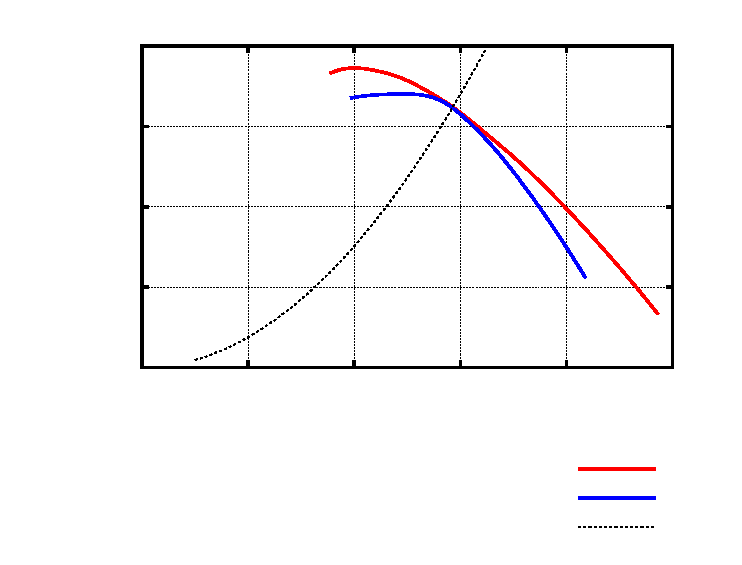
\includegraphics[width={340.10bp},height={255.10bp}]{PQ2}}%
    \gplfronttext
  \end{picture}%
\endgroup

	}
	\caption{Размерные характеристики сравниваемых вентиляторов}
	\label{fig:pq2}
\end{figure}

Безразмерные характеристики этих вентиляторов и сети показаны на рисунке \cref{fig:pq}. В рабочей точке, где пересекаются характеристика сети и характеристика вентилятора, ступени имеют совпадающие развиваемое давление \( P_\nu \) и производительность \(Q\) и имеют примерно одинаковый КПД, но, так как различаются зависимости \(\bar{H}(\bar{c}_{a})\), отличаются частоты вращения необходимые для развития требуемых \(P_{\nu}\) и \(Q\): \(n_1/n_2 = 1,5\), где \(n_{1,2}\) –-- частоты вращения первого и второго колеса.

\begin{figure}[h]
	\centerfloat{	
		% GNUPLOT: LaTeX picture with Postscript
\begingroup
  \makeatletter
  \providecommand\color[2][]{%
    \GenericError{(gnuplot) \space\space\space\@spaces}{%
      Package color not loaded in conjunction with
      terminal option `colourtext'%
    }{See the gnuplot documentation for explanation.%
    }{Either use 'blacktext' in gnuplot or load the package
      color.sty in LaTeX.}%
    \renewcommand\color[2][]{}%
  }%
  \providecommand\includegraphics[2][]{%
    \GenericError{(gnuplot) \space\space\space\@spaces}{%
      Package graphicx or graphics not loaded%
    }{See the gnuplot documentation for explanation.%
    }{The gnuplot epslatex terminal needs graphicx.sty or graphics.sty.}%
    \renewcommand\includegraphics[2][]{}%
  }%
  \providecommand\rotatebox[2]{#2}%
  \@ifundefined{ifGPcolor}{%
    \newif\ifGPcolor
    \GPcolorfalse
  }{}%
  \@ifundefined{ifGPblacktext}{%
    \newif\ifGPblacktext
    \GPblacktexttrue
  }{}%
  % define a \g@addto@macro without @ in the name:
  \let\gplgaddtomacro\g@addto@macro
  % define empty templates for all commands taking text:
  \gdef\gplbacktext{}%
  \gdef\gplfronttext{}%
  \makeatother
  \ifGPblacktext
    % no textcolor at all
    \def\colorrgb#1{}%
    \def\colorgray#1{}%
  \else
    % gray or color?
    \ifGPcolor
      \def\colorrgb#1{\color[rgb]{#1}}%
      \def\colorgray#1{\color[gray]{#1}}%
      \expandafter\def\csname LTw\endcsname{\color{white}}%
      \expandafter\def\csname LTb\endcsname{\color{black}}%
      \expandafter\def\csname LTa\endcsname{\color{black}}%
      \expandafter\def\csname LT0\endcsname{\color[rgb]{1,0,0}}%
      \expandafter\def\csname LT1\endcsname{\color[rgb]{0,1,0}}%
      \expandafter\def\csname LT2\endcsname{\color[rgb]{0,0,1}}%
      \expandafter\def\csname LT3\endcsname{\color[rgb]{1,0,1}}%
      \expandafter\def\csname LT4\endcsname{\color[rgb]{0,1,1}}%
      \expandafter\def\csname LT5\endcsname{\color[rgb]{1,1,0}}%
      \expandafter\def\csname LT6\endcsname{\color[rgb]{0,0,0}}%
      \expandafter\def\csname LT7\endcsname{\color[rgb]{1,0.3,0}}%
      \expandafter\def\csname LT8\endcsname{\color[rgb]{0.5,0.5,0.5}}%
    \else
      % gray
      \def\colorrgb#1{\color{black}}%
      \def\colorgray#1{\color[gray]{#1}}%
      \expandafter\def\csname LTw\endcsname{\color{white}}%
      \expandafter\def\csname LTb\endcsname{\color{black}}%
      \expandafter\def\csname LTa\endcsname{\color{black}}%
      \expandafter\def\csname LT0\endcsname{\color{black}}%
      \expandafter\def\csname LT1\endcsname{\color{black}}%
      \expandafter\def\csname LT2\endcsname{\color{black}}%
      \expandafter\def\csname LT3\endcsname{\color{black}}%
      \expandafter\def\csname LT4\endcsname{\color{black}}%
      \expandafter\def\csname LT5\endcsname{\color{black}}%
      \expandafter\def\csname LT6\endcsname{\color{black}}%
      \expandafter\def\csname LT7\endcsname{\color{black}}%
      \expandafter\def\csname LT8\endcsname{\color{black}}%
    \fi
  \fi
    \setlength{\unitlength}{0.0500bp}%
    \ifx\gptboxheight\undefined%
      \newlength{\gptboxheight}%
      \newlength{\gptboxwidth}%
      \newsavebox{\gptboxtext}%
    \fi%
    \setlength{\fboxrule}{0.5pt}%
    \setlength{\fboxsep}{1pt}%
    \definecolor{tbcol}{rgb}{1,1,1}%
\begin{picture}(6802.00,5102.00)%
    \gplgaddtomacro\gplbacktext{%
      \csname LTb\endcsname%%
      \put(1204,1736){\makebox(0,0)[r]{\strut{}$0$}}%
      \csname LTb\endcsname%%
      \put(1204,2764){\makebox(0,0)[r]{\strut{}$0,05$}}%
      \csname LTb\endcsname%%
      \put(1204,3793){\makebox(0,0)[r]{\strut{}$0,1$}}%
      \csname LTb\endcsname%%
      \put(1204,4821){\makebox(0,0)[r]{\strut{}$0,15$}}%
      \csname LTb\endcsname%%
      \put(1372,1456){\makebox(0,0){\strut{}$0$}}%
      \csname LTb\endcsname%%
      \put(2193,1456){\makebox(0,0){\strut{}$0,1$}}%
      \csname LTb\endcsname%%
      \put(3014,1456){\makebox(0,0){\strut{}$0,2$}}%
      \csname LTb\endcsname%%
      \put(3835,1456){\makebox(0,0){\strut{}$0,3$}}%
      \csname LTb\endcsname%%
      \put(4655,1456){\makebox(0,0){\strut{}$0,4$}}%
      \csname LTb\endcsname%%
      \put(5476,1456){\makebox(0,0){\strut{}$0,5$}}%
      \csname LTb\endcsname%%
      \put(6297,1456){\makebox(0,0){\strut{}$0,6$}}%
    }%
    \gplgaddtomacro\gplfronttext{%
      \csname LTb\endcsname%%
      \put(266,3278){\rotatebox{-270}{\makebox(0,0){\strut{}$\bar{H}$}}}%
      \put(3834,1036){\makebox(0,0){\strut{}$\bar{c}_a$}}%
      \csname LTb\endcsname%%
      \put(5226,763){\makebox(0,0)[r]{\strut{}вентилятор 1}}%
      \csname LTb\endcsname%%
      \put(5226,483){\makebox(0,0)[r]{\strut{}вентилятор 2}}%
      \csname LTb\endcsname%%
      \put(5226,203){\makebox(0,0)[r]{\strut{}сопротивление сети}}%
    }%
    \gplbacktext
    \put(0,0){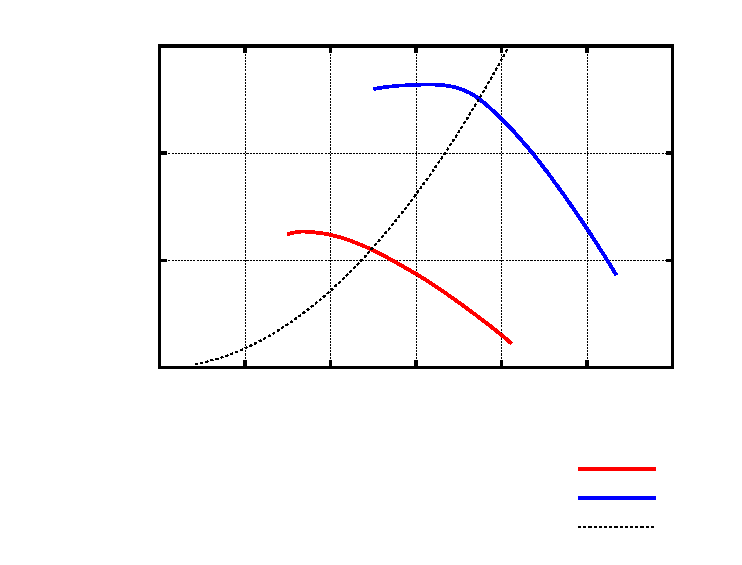
\includegraphics[width={340.10bp},height={255.10bp}]{PQ}}%
    \gplfronttext
  \end{picture}%
\endgroup

	}
	\caption{Безразмерные характеристики сравниваемых вентиляторов}
	\label{fig:pq}
\end{figure}

Механические нагрузки от действующих на лопатку центробежных сил зависят от квадрата частоты вращения рабочего колеса \(n\). При допущении, что лопатки рабочего колеса приблизительно одинаковы у первого и второго вентилятора, напряжения от сил растяжения в корневой части лопатки для второго вентилятора в \((n_1 / n_2)^2  = 2,25\) раз меньше, чем у первого. Однако при одинаковой потребляемой мощности момент на валу привода вентилятора возрастает пропорционально отношению частот вращения \(n_1 / n_2\), соответственно возрастают и механические нагрузки от аэродинамических сил.

Различающиеся частоты вращения приводят к изменениям и акустических характеристик. Разность между уровнями звуковой мощности вентиляторов можно оценить по формуле предложенной Е.Я. Юдиным \cite{Judin1964}:
\begin{equation}
	\Delta L_w=10\log\left[ \frac{\lambda_1(1-\eta_1)}{\lambda_2(1-\eta_2)}\left(\frac{U_\text{к1}}{U_\text{к2}}\right)^6\left(\frac{D_1}{D_2}\right)^2 \right],
	\label{eq:dLw}
\end{equation}
\begin{eqexpl}
	\item{\(\lambda\)} коэффициенты мощности вентиляторов: \(\lambda = 2\Ht\ca (1-\bar{d}^2)\);
	\item{\(\bar{d}\)} относительный диаметр втулки \(d\): \(\bar{d} = d / D\);
	\item{\(\eta\)} коэффициент полезного действия;
	\item{\(U_\text{к}\)} окружная скорость, м/с;
	\item{\(D\)} диаметр рабочего колеса, м.
	\end{eqexpl}

Для двух представленных вентиляторов с разной частотой  вращения разница мощности акустического излучения \( \Delta L_w \) по формуле \ref{eq:dLw} составляет приблизительно 5,3 дБ. 


\section{Ограничения на величину коэффициента теоретического напора}\label{ch1/sec3}

Типичные значения коэффициента теоретического напора \(\Ht\) осевого вентилятора или ступени компрессора находятся в пределах от 0,2 до 0,4 и редко превышают 0,45 при коэффициенте расхода \(\ca\) в диапазоне от 0,4 до 0,6. Влияние выбранных параметров \(\Ht\) и \(\ca\) на КПД $\eta$ компрессора иллюстрируется рисунком \cref{fig:etaFromHtCa} из работы \cite{Hall2012}. В границах типичных значений \(\Ht\) и \(\ca\) значение $\eta$ не сильно отличается от максимального и выход за типичные пределы значений, особенно в область высоких \(\Ht\), ведёт к резкому снижению КПД. Необходимые большие углы поворота потока требуют увеличения густоты решёток профилей и росту профильных потерь \cite{Howell1945, Bunimovich1967}. 
\begin{figure}[ht]
	\centerfloat{
		\begin{tabular}{m{0.5cm}m{240pt}}
			\multicolumn{1}{r}{\rotatebox{90}{$\Ht$}} & 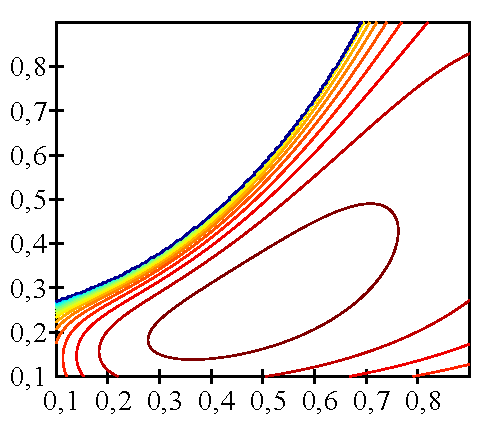
\includegraphics{images/11zon_cropped.pdf} \\
			& \multicolumn{1}{c}{$\ca$}\\
		\end{tabular}
	}
	\caption{Зависимость $\eta$ от сочетания параметров \(\Ht\) и \(\ca\) \cite{Hall2012}. Шаг между изолиниями 1\%; максимум 95\%}
	\label{fig:etaFromHtCa}
\end{figure}

В работе \cite{Dickens2011} исследовалась возможность применения высокого значения \(\Ht\) и его влияние на КПД ступени. При повышении \(\Ht\) с 0,45 до 0,55 адиабатический КПД ступени снизился примерно на 0,9\% и составил 86\%, а при повышении от 0,55 до 0,65 снизился ещё на 2,5\%. Коэффициент расхода \(\ca\) во всех случаях составлял 0,5. Рост потерь давления был связан с повышением толщины потери импульса $\delta_{2}$  на поверхностях лопатки. КПД спрямляющего аппарата оказался более чувствителен к изменению \(\Ht\), чем КПД рабочего колеса. Эффективное повышение \(\Ht\) потребовало увеличить степень реактивности ступени, то есть отношение работы сжатия в РК к работе сжатия во всей ступени.

Влияние выбора расчётных параметров \(\Ht\) и \(\ca\) на КПД вентилятора \(\eta\) для схемы состоящей из рабочего колеса и спрямляющего аппарата (РК+СА) можно оценить по графику \cref{fig:BrusEtaFromHtCa} из работы \cite{Brusilovskiy1986}. C ростом \(\Ht\) уменьшается $\eta$. Максимум $\eta$ так же снижается и смещается в сторону меньших \(\ca\), так как при б\'ольших \(\ca\) уменьшается \(\eta\) СА.
\begin{figure}[ht]
	\centerfloat{
		% GNUPLOT: LaTeX picture with Postscript
\begingroup
  \makeatletter
  \providecommand\color[2][]{%
    \GenericError{(gnuplot) \space\space\space\@spaces}{%
      Package color not loaded in conjunction with
      terminal option `colourtext'%
    }{See the gnuplot documentation for explanation.%
    }{Either use 'blacktext' in gnuplot or load the package
      color.sty in LaTeX.}%
    \renewcommand\color[2][]{}%
  }%
  \providecommand\includegraphics[2][]{%
    \GenericError{(gnuplot) \space\space\space\@spaces}{%
      Package graphicx or graphics not loaded%
    }{See the gnuplot documentation for explanation.%
    }{The gnuplot epslatex terminal needs graphicx.sty or graphics.sty.}%
    \renewcommand\includegraphics[2][]{}%
  }%
  \providecommand\rotatebox[2]{#2}%
  \@ifundefined{ifGPcolor}{%
    \newif\ifGPcolor
    \GPcolorfalse
  }{}%
  \@ifundefined{ifGPblacktext}{%
    \newif\ifGPblacktext
    \GPblacktexttrue
  }{}%
  % define a \g@addto@macro without @ in the name:
  \let\gplgaddtomacro\g@addto@macro
  % define empty templates for all commands taking text:
  \gdef\gplbacktext{}%
  \gdef\gplfronttext{}%
  \makeatother
  \ifGPblacktext
    % no textcolor at all
    \def\colorrgb#1{}%
    \def\colorgray#1{}%
  \else
    % gray or color?
    \ifGPcolor
      \def\colorrgb#1{\color[rgb]{#1}}%
      \def\colorgray#1{\color[gray]{#1}}%
      \expandafter\def\csname LTw\endcsname{\color{white}}%
      \expandafter\def\csname LTb\endcsname{\color{black}}%
      \expandafter\def\csname LTa\endcsname{\color{black}}%
      \expandafter\def\csname LT0\endcsname{\color[rgb]{1,0,0}}%
      \expandafter\def\csname LT1\endcsname{\color[rgb]{0,1,0}}%
      \expandafter\def\csname LT2\endcsname{\color[rgb]{0,0,1}}%
      \expandafter\def\csname LT3\endcsname{\color[rgb]{1,0,1}}%
      \expandafter\def\csname LT4\endcsname{\color[rgb]{0,1,1}}%
      \expandafter\def\csname LT5\endcsname{\color[rgb]{1,1,0}}%
      \expandafter\def\csname LT6\endcsname{\color[rgb]{0,0,0}}%
      \expandafter\def\csname LT7\endcsname{\color[rgb]{1,0.3,0}}%
      \expandafter\def\csname LT8\endcsname{\color[rgb]{0.5,0.5,0.5}}%
    \else
      % gray
      \def\colorrgb#1{\color{black}}%
      \def\colorgray#1{\color[gray]{#1}}%
      \expandafter\def\csname LTw\endcsname{\color{white}}%
      \expandafter\def\csname LTb\endcsname{\color{black}}%
      \expandafter\def\csname LTa\endcsname{\color{black}}%
      \expandafter\def\csname LT0\endcsname{\color{black}}%
      \expandafter\def\csname LT1\endcsname{\color{black}}%
      \expandafter\def\csname LT2\endcsname{\color{black}}%
      \expandafter\def\csname LT3\endcsname{\color{black}}%
      \expandafter\def\csname LT4\endcsname{\color{black}}%
      \expandafter\def\csname LT5\endcsname{\color{black}}%
      \expandafter\def\csname LT6\endcsname{\color{black}}%
      \expandafter\def\csname LT7\endcsname{\color{black}}%
      \expandafter\def\csname LT8\endcsname{\color{black}}%
    \fi
  \fi
    \setlength{\unitlength}{0.0500bp}%
    \ifx\gptboxheight\undefined%
      \newlength{\gptboxheight}%
      \newlength{\gptboxwidth}%
      \newsavebox{\gptboxtext}%
    \fi%
    \setlength{\fboxrule}{0.5pt}%
    \setlength{\fboxsep}{1pt}%
    \definecolor{tbcol}{rgb}{1,1,1}%
\begin{picture}(6802.00,5102.00)%
    \gplgaddtomacro\gplbacktext{%
      \csname LTb\endcsname%%
      \put(1204,1456){\makebox(0,0)[r]{\strut{}$0,8$}}%
      \csname LTb\endcsname%%
      \put(1204,2129){\makebox(0,0)[r]{\strut{}$0,82$}}%
      \csname LTb\endcsname%%
      \put(1204,2802){\makebox(0,0)[r]{\strut{}$0,84$}}%
      \csname LTb\endcsname%%
      \put(1204,3475){\makebox(0,0)[r]{\strut{}$0,86$}}%
      \csname LTb\endcsname%%
      \put(1204,4148){\makebox(0,0)[r]{\strut{}$0,88$}}%
      \csname LTb\endcsname%%
      \put(1204,4821){\makebox(0,0)[r]{\strut{}$0,9$}}%
      \csname LTb\endcsname%%
      \put(1372,1176){\makebox(0,0){\strut{}$0,4$}}%
      \csname LTb\endcsname%%
      \put(2193,1176){\makebox(0,0){\strut{}$0,5$}}%
      \csname LTb\endcsname%%
      \put(3014,1176){\makebox(0,0){\strut{}$0,6$}}%
      \csname LTb\endcsname%%
      \put(3834,1176){\makebox(0,0){\strut{}$0,7$}}%
      \csname LTb\endcsname%%
      \put(4655,1176){\makebox(0,0){\strut{}$0,8$}}%
      \csname LTb\endcsname%%
      \put(5476,1176){\makebox(0,0){\strut{}$0,9$}}%
      \csname LTb\endcsname%%
      \put(6297,1176){\makebox(0,0){\strut{}$1$}}%
    }%
    \gplgaddtomacro\gplfronttext{%
      \csname LTb\endcsname%%
      \put(266,3138){\rotatebox{-270}{\makebox(0,0){\strut{}$\eta$}}}%
      \put(3834,756){\makebox(0,0){\strut{}$\bar{c}_a$}}%
      \put(1500,320){\makebox(0,0){\strut{}$\bar{H}_\text{т}:$}}%
      \csname LTb\endcsname%%
      \put(2763,483){\makebox(0,0)[r]{\strut{}0,05}}%
      \csname LTb\endcsname%%
      \put(2763,203){\makebox(0,0)[r]{\strut{}0,1}}%
      \csname LTb\endcsname%%
      \put(4506,483){\makebox(0,0)[r]{\strut{}0,2}}%
      \csname LTb\endcsname%%
      \put(4506,203){\makebox(0,0)[r]{\strut{}0,4}}%
    }%
    \gplbacktext
    \put(0,0){\includegraphics[width={340.10bp},height={255.10bp}]{BrusEta}}%
    \gplfronttext
  \end{picture}%
\endgroup

	}
	\caption{Зависимость $\eta$ схемы РК+СА от расчётных значений \(\Ht\)~и~\(\ca\)}
	\label{fig:BrusEtaFromHtCa}
\end{figure}
\section{Пределы аэродинамической нагруженности}\label{ch1/sec4}

Для течения в лопаточных венцах вентилятора характерно существование таких режимов работы, при которых происходит образование отрывных зон приводящих к резкому снижению КПД. Близость режима возникновения отрыва потока в проточной части вентилятора к его расчетному режиму характеризуется аэродинамической нагруженностью лопаточных венцов. Для различных элементов проточной части отличаются факторы возникновения и механизмы развития отрыва. Для оценки аэродинамической нагруженности по каждому из факторов разработаны отдельные критерии.

\subsection{Вязкий отрыв пограничного слоя}\label{ch1/sec5}

Отрыв потока от поверхностей лопатки и элементов проточной части вентилятора обусловленный вязкостью воздуха происходит в связи с наличием пограничного слоя. На жидкие частицы в пограничном слое действуют значительные касательные напряжения, при приближении к поверхности происходит резкое снижение скорости и кинетической энергии. При диффузорном течении статическое давление увеличивается по ходу движения газа, и пристеночные слои воздуха подтормаживаются сильнее, пока им достаточно энергии для преодоления градиента давления, после чего останавливаются. В точке остановки слоя воздуха происходит отрыв пограничного слоя от поверхности, ниже по течению появляются области обратного течения, основной поток отходит от поверхности и ускоряется, что приводит к росту потерь полного давления. 

Для оценки аэродинамической нагруженности с точки зрения вязкого отрыва пограничного слоя потока в решетках профилей разными авторами был предложен ряд критериев. К примеру, величина произведения густоты решётки на коэффициент подъёмной силы профиля $\tau C_y$ \cite{Hausenblas1963,Dovjik1968} и угол раскрытия эквивалентного диффузора \(\gamma\) \cite{Dovjik1958,Uschakov1963}. Большое распространение получил фактор эквивалентной диффузорности Либляйна \cite{Lieblein1959}:
\begin{equation}
	D_\text{eq} = \frac{\cos \beta_2}{\cos \beta_1} \left[ 1,12 + 0,61\frac{\cos^2\beta_1}{\tau}(\tan \beta_1 - \tan\beta_2) \right],
	\label{eq:DeqLieblein}
\end{equation}
\begin{eqexpl}
	\item{$\beta_{1,2}$} угол между скоростью потока в относительном движении перед (1) и за (2) решёткой профилей и осью решетки;
	\item{$\tau$} густота решетки.
\end{eqexpl}

Этот фактор разработан для плоских решёток составленных из профилей NACA"--~65 работающих на режиме минимальных потерь, но применяется для широкого класса задач. Либляйн применил его при анализе материалов экспериментальных продувок решёток профилей с углом атаки превышающем угол соответствующий режиму работы решётки с минимальным уровнем потерь (рисунок \ref{fig:DeqLieblein}). Был установлен резкий рост толщины потери импульса $\delta_2$ и отрыв потока при превышении величины $D_\text{eq}$ значения приблизительно равного 2 \cite{Lieblein1959}. При предварительном профилировании лопаток осевого вентилятора, благодаря простоте выражения \ref{eq:DeqLieblein}, удобно использовать $D_\text{eq}$ при анализе вариантов геометрии.
\begin{figure}[ht]
\centerfloat{
\begin{tabular}{m{0.5cm}m{12cm}}
\multicolumn{1}{r}{\rotatebox{90}{$\delta_2/c$}} & 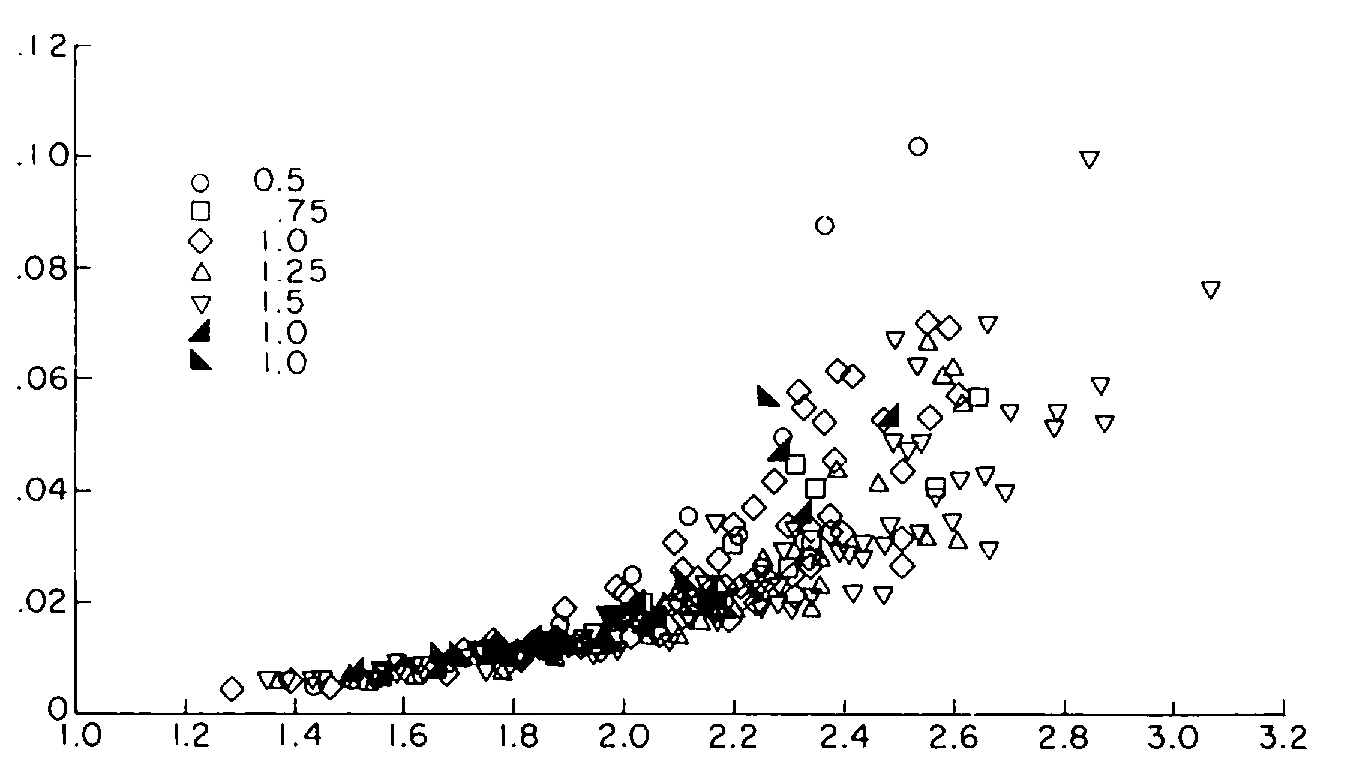
\includegraphics{images/DeqLeiblein.png} \\
   & \multicolumn{1}{c}{$D_\text{eq}$}\\
\end{tabular}	
}
	\caption{Рост толщины потери импульса отнесённой к хорде профиля~$\delta_2/c$ в зависимости от $D_\text{eq}$ \cite{Lieblein1959}}
	\label{fig:DeqLieblein}
\end{figure}

Течение в лопаточных венцах вентиляторов отличается от течения в плоских решётках, которое часто рассматривается при упрощении. Особенно значительные отличия проявляются в концевых областях, где взаимодействуют пограничные слои на лопатках и торцевых поверхностях вызывая вторичные течения. 
Во вращающихся венцах характер вторичных течений изменяется под действием центробежных сил на пограничный слой. Заторможенные в пограничном слое лопатки жидкие частицы перемещаются к периферии. В привтулочных сечениях лопатки влияние пограничного слоя ослабляется, а в периферийных, наоборот, усиливается. Соответственно меняется и аэродинамическая нагруженность в сравнении с нагруженностью плоской решётки \cite{Brusilovskiy1986}. Это позволяет выбирать несколько меньшую густоту решётки у втулки и большую у периферии, чем это следует из обобщённых продувок плоских решёток профилей.

\subsection{Потеря устойчивости вращающегося потока}\label{ch1/sec6}

В закрученных потоках давление уменьшается в направлении от периферии к оси вращения. На жидкие частицы в разных направлениях действуют силы инерции и силы давления, что обеспечивает радиальное равновесие \cite{Smith1966}. При достаточной интенсивности закрутки равновесие нарушается, в приосевой части течения возможно образование замкнутых циркуляционных зон. При проектировании ряда устройств, к примеру вихревых горелках или циклонных сепараторах, образование таких зон заложено намерено для стабилизации пламени, обеспечения полноты сгорания или разделения фракций разной плотности \cite{Gupta1987, Goldschtik1981}.
Ключевым критерием подобия в закрученных течениях является параметр закрутки \(S\):
\begin{equation}
	S = \frac{G_\theta}{G_x R},
	\label{eq:S}
\end{equation}
\begin{eqexpl}
	\item{\(G_\theta\)} поток момента количества движения, \(\si\kilogram\cdot\si\meter^2/\si\second^2\);
	\item{\(G_x\)} поток количества движения, \(\si\kilogram\cdot\si\meter/\si\second^2\);
	\item{\(R\)} радиус сопла, \(\si\meter\).
\end{eqexpl}

В турбомашинах так же могут возникать циркуляционные зоны, например, в последних ступенях паровых турбин \cite{Bammert1949} или в осевых вентиляторах с большой долей статического давления в полном \cite{Mitrofovich1991}. Незапланированные зоны отрыва ведут к изменению структуры потока и нарушению нормальной работы машины. Циркуляционные зоны (рисунок \ref{fig:Mitrof1999}) при таком типе отрыва начинают развитие у выходной кромки втулки и распространяются вверх по потоку, увеличивая свои размеры и интенсивность, являясь при этом нестационарными и вращающимися в направлении закрутки потока \cite{Mitrofovich1999}. 
\begin{figure} [ht]
	\centerfloat{
		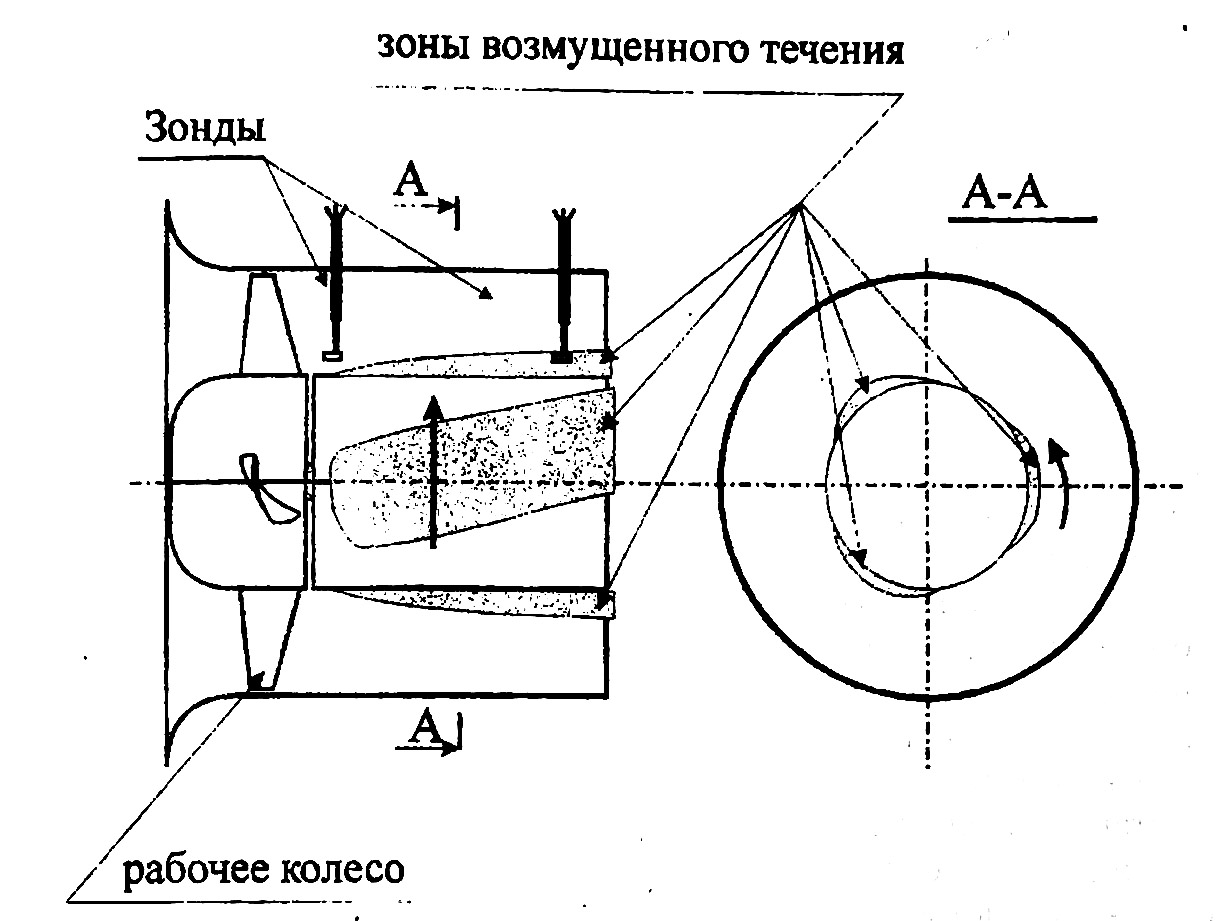
\includegraphics[width=12cm,keepaspectratio]{images/Mitrof1999}
	}
		\caption{Схема отрывных зон при потери устойчивости течения у втулки за осевым вентилятором \cite{Mitrofovich1999}}
	\label{fig:Mitrof1999}
\end{figure}

Для вентилятора состоящему только из рабочего колеса спрофилированного по закону постоянной циркуляции (\(C_u r = \text{const}\)), используется обратный критерий записанный через безразмерные параметры \(\bar{d}\ca/\Ht\). Опираясь на это число, можно определить радиус циркуляционной зоны, возникающей при распаде вихря при течении в трубе \cite{Strscheletzky1955}. В зависимости от кинематики потока и геометрии проточной части вентилятора циркуляционные зоны возникают вместе с отрывом потока от поверхности втулки \cite{Mitrofovich1991}, граница допустимых сочетаний параметров показана на графике \ref{fig:RoMitrof}. 
\begin{figure} [ht]
	\centerfloat{
	 % GNUPLOT: LaTeX picture with Postscript
\begingroup
  \makeatletter
  \providecommand\color[2][]{%
    \GenericError{(gnuplot) \space\space\space\@spaces}{%
      Package color not loaded in conjunction with
      terminal option `colourtext'%
    }{See the gnuplot documentation for explanation.%
    }{Either use 'blacktext' in gnuplot or load the package
      color.sty in LaTeX.}%
    \renewcommand\color[2][]{}%
  }%
  \providecommand\includegraphics[2][]{%
    \GenericError{(gnuplot) \space\space\space\@spaces}{%
      Package graphicx or graphics not loaded%
    }{See the gnuplot documentation for explanation.%
    }{The gnuplot epslatex terminal needs graphicx.sty or graphics.sty.}%
    \renewcommand\includegraphics[2][]{}%
  }%
  \providecommand\rotatebox[2]{#2}%
  \@ifundefined{ifGPcolor}{%
    \newif\ifGPcolor
    \GPcolorfalse
  }{}%
  \@ifundefined{ifGPblacktext}{%
    \newif\ifGPblacktext
    \GPblacktexttrue
  }{}%
  % define a \g@addto@macro without @ in the name:
  \let\gplgaddtomacro\g@addto@macro
  % define empty templates for all commands taking text:
  \gdef\gplbacktext{}%
  \gdef\gplfronttext{}%
  \makeatother
  \ifGPblacktext
    % no textcolor at all
    \def\colorrgb#1{}%
    \def\colorgray#1{}%
  \else
    % gray or color?
    \ifGPcolor
      \def\colorrgb#1{\color[rgb]{#1}}%
      \def\colorgray#1{\color[gray]{#1}}%
      \expandafter\def\csname LTw\endcsname{\color{white}}%
      \expandafter\def\csname LTb\endcsname{\color{black}}%
      \expandafter\def\csname LTa\endcsname{\color{black}}%
      \expandafter\def\csname LT0\endcsname{\color[rgb]{1,0,0}}%
      \expandafter\def\csname LT1\endcsname{\color[rgb]{0,1,0}}%
      \expandafter\def\csname LT2\endcsname{\color[rgb]{0,0,1}}%
      \expandafter\def\csname LT3\endcsname{\color[rgb]{1,0,1}}%
      \expandafter\def\csname LT4\endcsname{\color[rgb]{0,1,1}}%
      \expandafter\def\csname LT5\endcsname{\color[rgb]{1,1,0}}%
      \expandafter\def\csname LT6\endcsname{\color[rgb]{0,0,0}}%
      \expandafter\def\csname LT7\endcsname{\color[rgb]{1,0.3,0}}%
      \expandafter\def\csname LT8\endcsname{\color[rgb]{0.5,0.5,0.5}}%
    \else
      % gray
      \def\colorrgb#1{\color{black}}%
      \def\colorgray#1{\color[gray]{#1}}%
      \expandafter\def\csname LTw\endcsname{\color{white}}%
      \expandafter\def\csname LTb\endcsname{\color{black}}%
      \expandafter\def\csname LTa\endcsname{\color{black}}%
      \expandafter\def\csname LT0\endcsname{\color{black}}%
      \expandafter\def\csname LT1\endcsname{\color{black}}%
      \expandafter\def\csname LT2\endcsname{\color{black}}%
      \expandafter\def\csname LT3\endcsname{\color{black}}%
      \expandafter\def\csname LT4\endcsname{\color{black}}%
      \expandafter\def\csname LT5\endcsname{\color{black}}%
      \expandafter\def\csname LT6\endcsname{\color{black}}%
      \expandafter\def\csname LT7\endcsname{\color{black}}%
      \expandafter\def\csname LT8\endcsname{\color{black}}%
    \fi
  \fi
    \setlength{\unitlength}{0.0500bp}%
    \ifx\gptboxheight\undefined%
      \newlength{\gptboxheight}%
      \newlength{\gptboxwidth}%
      \newsavebox{\gptboxtext}%
    \fi%
    \setlength{\fboxrule}{0.5pt}%
    \setlength{\fboxsep}{1pt}%
    \definecolor{tbcol}{rgb}{1,1,1}%
\begin{picture}(6802.00,5102.00)%
    \gplgaddtomacro\gplbacktext{%
      \csname LTb\endcsname%%
      \put(1036,896){\makebox(0,0)[r]{\strut{}$0,4$}}%
      \csname LTb\endcsname%%
      \put(1036,1877){\makebox(0,0)[r]{\strut{}$0,6$}}%
      \csname LTb\endcsname%%
      \put(1036,2859){\makebox(0,0)[r]{\strut{}$0,8$}}%
      \csname LTb\endcsname%%
      \put(1036,3840){\makebox(0,0)[r]{\strut{}$1$}}%
      \csname LTb\endcsname%%
      \put(1036,4821){\makebox(0,0)[r]{\strut{}$1,2$}}%
      \csname LTb\endcsname%%
      \put(1204,616){\makebox(0,0){\strut{}$1$}}%
      \csname LTb\endcsname%%
      \put(2053,616){\makebox(0,0){\strut{}$1,5$}}%
      \csname LTb\endcsname%%
      \put(2902,616){\makebox(0,0){\strut{}$2$}}%
      \csname LTb\endcsname%%
      \put(3751,616){\makebox(0,0){\strut{}$2,5$}}%
      \csname LTb\endcsname%%
      \put(4599,616){\makebox(0,0){\strut{}$3$}}%
      \csname LTb\endcsname%%
      \put(5448,616){\makebox(0,0){\strut{}$3,5$}}%
      \csname LTb\endcsname%%
      \put(6297,616){\makebox(0,0){\strut{}$4$}}%
    }%
    \gplgaddtomacro\gplfronttext{%
      \csname LTb\endcsname%%
      \put(266,2858){\rotatebox{-270}{\makebox(0,0){\strut{}$\bar{d}\ca/\Ht$}}}%
      \put(3750,196){\makebox(0,0){\strut{}$\tan \beta_1$}}%
    }%
    \gplbacktext
    \put(0,0){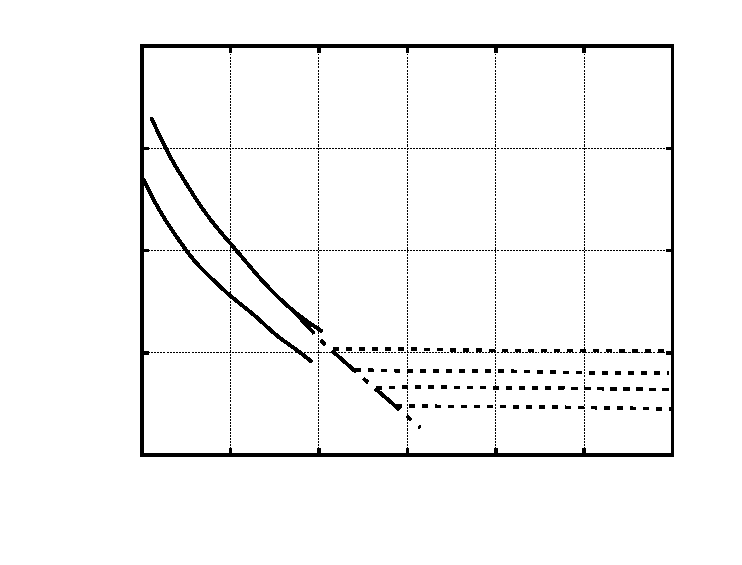
\includegraphics[width={340.10bp},height={255.10bp}]{Mitrof1991}}%
    \gplfronttext
  \end{picture}%
\endgroup

	 
	 \begin{eqexpl}
	 	\item{\(\beta_1\)} угол между направлением скорости потока перед решёткой и осью решётки;
	 \end{eqexpl}
	}
	\caption{Границы существования высокоэффективных вентиляторов различных аэродинамических схем \cite{Mitrofovich1991}}
	\label{fig:RoMitrof}
\end{figure}

\subsection{Методы снижения аэродинамической нагруженности}\label{ch1/sec7}

С целью повышения эффективности или расширения диапазона рабочих режимов для улучшения аэродинамических или эксплуатационных характеристик машин и аппаратов производится управление пограничным слоем. Управление производится в виде уменьшения влияния пограничного слоя на течение, путём либо изменения формы тела так, чтобы сохранить высокий уровень энергии вблизи поверхности, либо повышения уровня энергии с помощью дополнительных устройств. Широкий обзор методов управления отрывом потока дан в монографии  \cite{Chen1979}.

В высоконагруженных ступенях осевых вентиляторов наличие небольших локальных отрывных пузырей на поверхности лопатки у втулки и у задней кромки не оказывает значительного негативного влияния на аэродинамические характеристики. С точки зрения эффективности выгоднее лишь ослабить влияние отрывных зон чем полностью их ликвидировать \cite{Chen1979}.

Течение в диффузорных решётках сопряжено с градиентом давления на спинке профилей и возможностью отрыва потока. Управление пограничным слоем с помощью специального профилирования \cite{Papailiou1970,Hobbs1984,Meng2023}, обеспечивающего предварительно заданное распределение давления на спинке профиля, позволяет снижать профильные потери полного давления. Контроль над местом ламинарно-турбулентного перехода и состоянием пограничного слоя снижает аэродинамическую нагруженность решётки и позволяет выбирать меньшие густоты, чем при использовании обычных серий профилей. Однако такие профили требуют повышенной точности исполнения.

Главное преимущество такого подхода к профилированию заключается в том, чтобы снизить максимальные местные числа Маха на спинке профиля для предотвращения возникновения локальных скачков уплотнения, повышающих потери давления и провоцирующих отрыв пограничного слоя. В работе \cite{Hobbs1984} для одного режима работы двух решёток профилей приведено сравнение коэффициента потерь полного давления \(\zeta = \Delta P /0,5 \rho W_1^2\), (где \(\Delta P\) "--- потери полного давления, Па; \(W_1\) "--- скорость перед решёткой, \(\si\meter/\si\second\)) в зависимости от числа Маха на входе в решётку \(M_1\) (рисунок \ref{fig:Hobbs1984}). Профили первой решётки были специально спрофилированы, вторые выбраны из серии профилей NACA-400. Специальное профилирование позволило получить меньшие потери при умеренных числах \(M_1\) до 0,7, и большее критическое число Маха, при котором потери начинают резко расти. 
\begin{figure} [ht]
	\centerfloat{
		% GNUPLOT: LaTeX picture with Postscript
\begingroup
  \makeatletter
  \providecommand\color[2][]{%
    \GenericError{(gnuplot) \space\space\space\@spaces}{%
      Package color not loaded in conjunction with
      terminal option `colourtext'%
    }{See the gnuplot documentation for explanation.%
    }{Either use 'blacktext' in gnuplot or load the package
      color.sty in LaTeX.}%
    \renewcommand\color[2][]{}%
  }%
  \providecommand\includegraphics[2][]{%
    \GenericError{(gnuplot) \space\space\space\@spaces}{%
      Package graphicx or graphics not loaded%
    }{See the gnuplot documentation for explanation.%
    }{The gnuplot epslatex terminal needs graphicx.sty or graphics.sty.}%
    \renewcommand\includegraphics[2][]{}%
  }%
  \providecommand\rotatebox[2]{#2}%
  \@ifundefined{ifGPcolor}{%
    \newif\ifGPcolor
    \GPcolorfalse
  }{}%
  \@ifundefined{ifGPblacktext}{%
    \newif\ifGPblacktext
    \GPblacktexttrue
  }{}%
  % define a \g@addto@macro without @ in the name:
  \let\gplgaddtomacro\g@addto@macro
  % define empty templates for all commands taking text:
  \gdef\gplbacktext{}%
  \gdef\gplfronttext{}%
  \makeatother
  \ifGPblacktext
    % no textcolor at all
    \def\colorrgb#1{}%
    \def\colorgray#1{}%
  \else
    % gray or color?
    \ifGPcolor
      \def\colorrgb#1{\color[rgb]{#1}}%
      \def\colorgray#1{\color[gray]{#1}}%
      \expandafter\def\csname LTw\endcsname{\color{white}}%
      \expandafter\def\csname LTb\endcsname{\color{black}}%
      \expandafter\def\csname LTa\endcsname{\color{black}}%
      \expandafter\def\csname LT0\endcsname{\color[rgb]{1,0,0}}%
      \expandafter\def\csname LT1\endcsname{\color[rgb]{0,1,0}}%
      \expandafter\def\csname LT2\endcsname{\color[rgb]{0,0,1}}%
      \expandafter\def\csname LT3\endcsname{\color[rgb]{1,0,1}}%
      \expandafter\def\csname LT4\endcsname{\color[rgb]{0,1,1}}%
      \expandafter\def\csname LT5\endcsname{\color[rgb]{1,1,0}}%
      \expandafter\def\csname LT6\endcsname{\color[rgb]{0,0,0}}%
      \expandafter\def\csname LT7\endcsname{\color[rgb]{1,0.3,0}}%
      \expandafter\def\csname LT8\endcsname{\color[rgb]{0.5,0.5,0.5}}%
    \else
      % gray
      \def\colorrgb#1{\color{black}}%
      \def\colorgray#1{\color[gray]{#1}}%
      \expandafter\def\csname LTw\endcsname{\color{white}}%
      \expandafter\def\csname LTb\endcsname{\color{black}}%
      \expandafter\def\csname LTa\endcsname{\color{black}}%
      \expandafter\def\csname LT0\endcsname{\color{black}}%
      \expandafter\def\csname LT1\endcsname{\color{black}}%
      \expandafter\def\csname LT2\endcsname{\color{black}}%
      \expandafter\def\csname LT3\endcsname{\color{black}}%
      \expandafter\def\csname LT4\endcsname{\color{black}}%
      \expandafter\def\csname LT5\endcsname{\color{black}}%
      \expandafter\def\csname LT6\endcsname{\color{black}}%
      \expandafter\def\csname LT7\endcsname{\color{black}}%
      \expandafter\def\csname LT8\endcsname{\color{black}}%
    \fi
  \fi
    \setlength{\unitlength}{0.0500bp}%
    \ifx\gptboxheight\undefined%
      \newlength{\gptboxheight}%
      \newlength{\gptboxwidth}%
      \newsavebox{\gptboxtext}%
    \fi%
    \setlength{\fboxrule}{0.5pt}%
    \setlength{\fboxsep}{1pt}%
    \definecolor{tbcol}{rgb}{1,1,1}%
\begin{picture}(6802.00,5102.00)%
    \gplgaddtomacro\gplbacktext{%
      \csname LTb\endcsname%%
      \put(1204,1456){\makebox(0,0)[r]{\strut{}$0,01$}}%
      \csname LTb\endcsname%%
      \put(1204,2017){\makebox(0,0)[r]{\strut{}$0,02$}}%
      \csname LTb\endcsname%%
      \put(1204,2578){\makebox(0,0)[r]{\strut{}$0,03$}}%
      \csname LTb\endcsname%%
      \put(1204,3139){\makebox(0,0)[r]{\strut{}$0,04$}}%
      \csname LTb\endcsname%%
      \put(1204,3699){\makebox(0,0)[r]{\strut{}$0,05$}}%
      \csname LTb\endcsname%%
      \put(1204,4260){\makebox(0,0)[r]{\strut{}$0,06$}}%
      \csname LTb\endcsname%%
      \put(1204,4821){\makebox(0,0)[r]{\strut{}$0,07$}}%
      \csname LTb\endcsname%%
      \put(1372,1176){\makebox(0,0){\strut{}$0,3$}}%
      \csname LTb\endcsname%%
      \put(2193,1176){\makebox(0,0){\strut{}$0,4$}}%
      \csname LTb\endcsname%%
      \put(3014,1176){\makebox(0,0){\strut{}$0,5$}}%
      \csname LTb\endcsname%%
      \put(3834,1176){\makebox(0,0){\strut{}$0,6$}}%
      \csname LTb\endcsname%%
      \put(4655,1176){\makebox(0,0){\strut{}$0,7$}}%
      \csname LTb\endcsname%%
      \put(5476,1176){\makebox(0,0){\strut{}$0,8$}}%
      \csname LTb\endcsname%%
      \put(6297,1176){\makebox(0,0){\strut{}$0,9$}}%
    }%
    \gplgaddtomacro\gplfronttext{%
      \csname LTb\endcsname%%
      \put(266,3138){\rotatebox{-270}{\makebox(0,0){\strut{}$\zeta$}}}%
      \put(3834,756){\makebox(0,0){\strut{}$M_1$}}%
      \csname LTb\endcsname%%
      \put(5226,483){\makebox(0,0)[r]{\strut{}специальное профилирование}}%
      \csname LTb\endcsname%%
      \put(5226,203){\makebox(0,0)[r]{\strut{}профили NACA-405}}%
    }%
    \gplbacktext
    \put(0,0){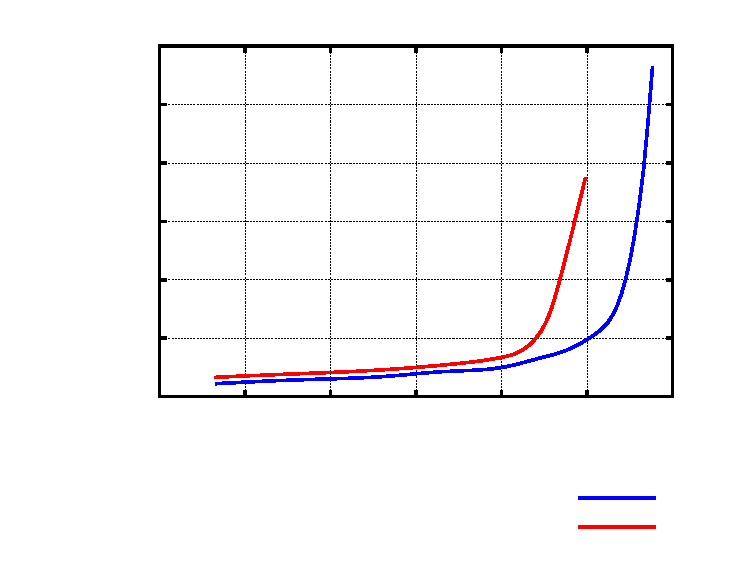
\includegraphics[width={340.10bp},height={255.10bp}]{Hobbs1984}}%
    \gplfronttext
  \end{picture}%
\endgroup

	}
	\caption{Сопоставление коэффициента потерь \(\zeta\) в решётках с профилями с специальным профилированием и серии NACA-400 при разных числах маха на входе \(M_1\) \cite{Hobbs1984}}
	\label{fig:Hobbs1984}
\end{figure}

Широкое исследование методов аэродинамического совершенствования высоконагруженных лопаточных аппаратов компрессоров выполнено в работе \cite{Tereschenko1988}. Рассматриваются активные методы управления пограничным слоем такие как вдув струй в пограничный слой, отсос пограничного слоя и пассивные, такие как применение двухрядных решёток и трубулизаторов  потока (рисунок \ref{fig:Tereshenko1988}).

\begin{figure} [ht]
\centerfloat{
	\subcaptionbox[teresh]{вдув в пограничный слой}{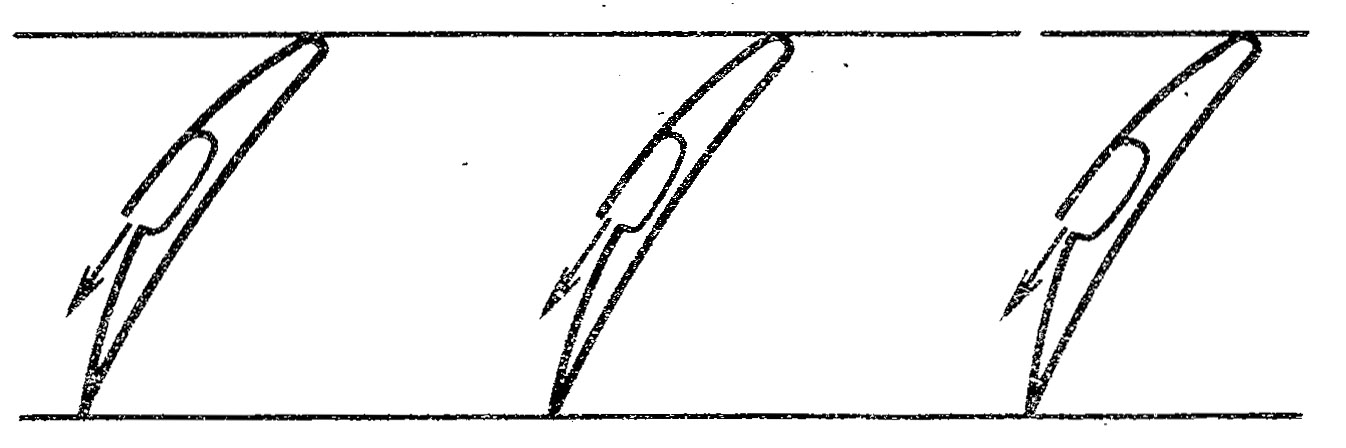
\includegraphics[width=8cm,keepaspectratio]{images/tereshenko1988a}}
	\hfill
	\subcaptionbox{отсос пограничного слоя}{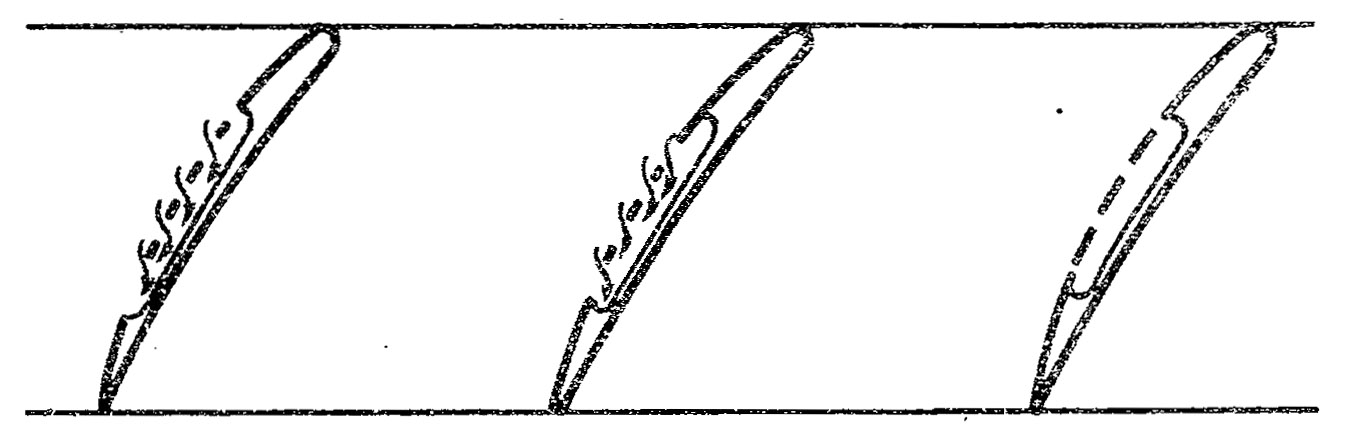
\includegraphics[width=8cm,keepaspectratio]{images/tereshenko1988b}}
\hfill
	\subcaptionbox{многорядные решётки}{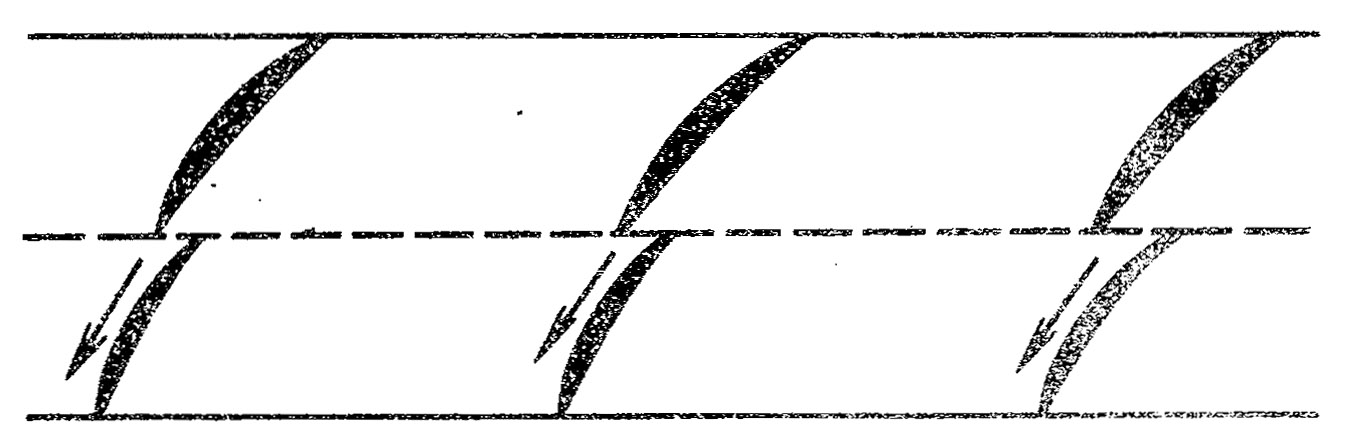
\includegraphics[width=8cm,keepaspectratio]{images/tereshenko1988c}}
\hfill
	\subcaptionbox{профили с турбулизаторами}{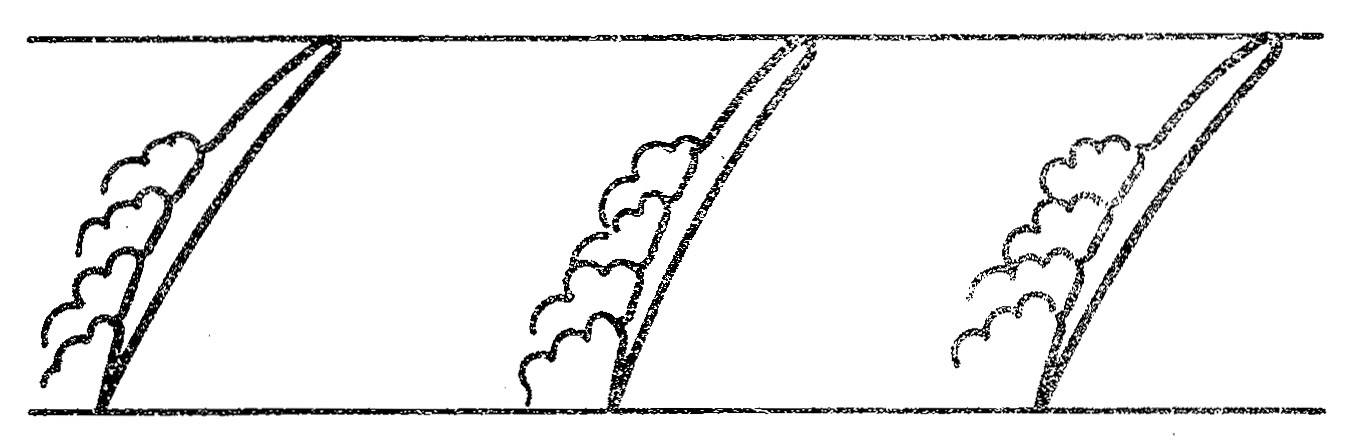
\includegraphics[width=8cm,keepaspectratio]{images/tereshenko1988d}}
}
\caption{Схемы управления обтеканием лопаток в решётках \cite{Tereschenko1988}}
\label{fig:Tereshenko1988}
\end{figure}

Активные методы управления пограничным слоем вдувом и отсосом газа с поверхности лопатки не нашли распространения в компрессорах и вентиляторах в связи с конструктивной сложностью. Наиболее простым методом является пассивный метод турбулизации потока, суть которого заключается в уменьшении участка ламинарного пограничного слоя на лопатке для снижения вероятности его отрыва. На рисунке \ref{fig:Tereschenko1988turb} сравнение степени повышения давления приведённой к расчётной \(\bar{\pi}_\text{ст}\) в ступени с гладкими лопатками и турбулизаторами потока в зависимости от приведённого расхода \(\bar{G}\) для разных приведённых частот вращения \(\bar{n}\). Применение турбулизатора позволило расширить область работы в сторону меньших расходов, но заметно снизило \(\bar{\pi}_\text{ст}\).
\begin{figure} [ht]
	\centerfloat{
		%\includegraphics[width=8cm,keepaspectratio]{images/tereshenko1988turb},
		% GNUPLOT: LaTeX picture with Postscript
\begingroup
  \makeatletter
  \providecommand\color[2][]{%
    \GenericError{(gnuplot) \space\space\space\@spaces}{%
      Package color not loaded in conjunction with
      terminal option `colourtext'%
    }{See the gnuplot documentation for explanation.%
    }{Either use 'blacktext' in gnuplot or load the package
      color.sty in LaTeX.}%
    \renewcommand\color[2][]{}%
  }%
  \providecommand\includegraphics[2][]{%
    \GenericError{(gnuplot) \space\space\space\@spaces}{%
      Package graphicx or graphics not loaded%
    }{See the gnuplot documentation for explanation.%
    }{The gnuplot epslatex terminal needs graphicx.sty or graphics.sty.}%
    \renewcommand\includegraphics[2][]{}%
  }%
  \providecommand\rotatebox[2]{#2}%
  \@ifundefined{ifGPcolor}{%
    \newif\ifGPcolor
    \GPcolorfalse
  }{}%
  \@ifundefined{ifGPblacktext}{%
    \newif\ifGPblacktext
    \GPblacktexttrue
  }{}%
  % define a \g@addto@macro without @ in the name:
  \let\gplgaddtomacro\g@addto@macro
  % define empty templates for all commands taking text:
  \gdef\gplbacktext{}%
  \gdef\gplfronttext{}%
  \makeatother
  \ifGPblacktext
    % no textcolor at all
    \def\colorrgb#1{}%
    \def\colorgray#1{}%
  \else
    % gray or color?
    \ifGPcolor
      \def\colorrgb#1{\color[rgb]{#1}}%
      \def\colorgray#1{\color[gray]{#1}}%
      \expandafter\def\csname LTw\endcsname{\color{white}}%
      \expandafter\def\csname LTb\endcsname{\color{black}}%
      \expandafter\def\csname LTa\endcsname{\color{black}}%
      \expandafter\def\csname LT0\endcsname{\color[rgb]{1,0,0}}%
      \expandafter\def\csname LT1\endcsname{\color[rgb]{0,1,0}}%
      \expandafter\def\csname LT2\endcsname{\color[rgb]{0,0,1}}%
      \expandafter\def\csname LT3\endcsname{\color[rgb]{1,0,1}}%
      \expandafter\def\csname LT4\endcsname{\color[rgb]{0,1,1}}%
      \expandafter\def\csname LT5\endcsname{\color[rgb]{1,1,0}}%
      \expandafter\def\csname LT6\endcsname{\color[rgb]{0,0,0}}%
      \expandafter\def\csname LT7\endcsname{\color[rgb]{1,0.3,0}}%
      \expandafter\def\csname LT8\endcsname{\color[rgb]{0.5,0.5,0.5}}%
    \else
      % gray
      \def\colorrgb#1{\color{black}}%
      \def\colorgray#1{\color[gray]{#1}}%
      \expandafter\def\csname LTw\endcsname{\color{white}}%
      \expandafter\def\csname LTb\endcsname{\color{black}}%
      \expandafter\def\csname LTa\endcsname{\color{black}}%
      \expandafter\def\csname LT0\endcsname{\color{black}}%
      \expandafter\def\csname LT1\endcsname{\color{black}}%
      \expandafter\def\csname LT2\endcsname{\color{black}}%
      \expandafter\def\csname LT3\endcsname{\color{black}}%
      \expandafter\def\csname LT4\endcsname{\color{black}}%
      \expandafter\def\csname LT5\endcsname{\color{black}}%
      \expandafter\def\csname LT6\endcsname{\color{black}}%
      \expandafter\def\csname LT7\endcsname{\color{black}}%
      \expandafter\def\csname LT8\endcsname{\color{black}}%
    \fi
  \fi
    \setlength{\unitlength}{0.0500bp}%
    \ifx\gptboxheight\undefined%
      \newlength{\gptboxheight}%
      \newlength{\gptboxwidth}%
      \newsavebox{\gptboxtext}%
    \fi%
    \setlength{\fboxrule}{0.5pt}%
    \setlength{\fboxsep}{1pt}%
    \definecolor{tbcol}{rgb}{1,1,1}%
\begin{picture}(6802.00,5102.00)%
    \gplgaddtomacro\gplbacktext{%
      \csname LTb\endcsname%%
      \put(1036,1456){\makebox(0,0)[r]{\strut{}$0,6$}}%
      \csname LTb\endcsname%%
      \put(1036,2129){\makebox(0,0)[r]{\strut{}$0,7$}}%
      \csname LTb\endcsname%%
      \put(1036,2802){\makebox(0,0)[r]{\strut{}$0,8$}}%
      \csname LTb\endcsname%%
      \put(1036,3475){\makebox(0,0)[r]{\strut{}$0,9$}}%
      \csname LTb\endcsname%%
      \put(1036,4148){\makebox(0,0)[r]{\strut{}$1$}}%
      \csname LTb\endcsname%%
      \put(1036,4821){\makebox(0,0)[r]{\strut{}$1,1$}}%
      \csname LTb\endcsname%%
      \put(1204,1176){\makebox(0,0){\strut{}$0,4$}}%
      \csname LTb\endcsname%%
      \put(1841,1176){\makebox(0,0){\strut{}$0,5$}}%
      \csname LTb\endcsname%%
      \put(2477,1176){\makebox(0,0){\strut{}$0,6$}}%
      \csname LTb\endcsname%%
      \put(3114,1176){\makebox(0,0){\strut{}$0,7$}}%
      \csname LTb\endcsname%%
      \put(3750,1176){\makebox(0,0){\strut{}$0,8$}}%
      \csname LTb\endcsname%%
      \put(4387,1176){\makebox(0,0){\strut{}$0,9$}}%
      \csname LTb\endcsname%%
      \put(5024,1176){\makebox(0,0){\strut{}$1$}}%
      \csname LTb\endcsname%%
      \put(5660,1176){\makebox(0,0){\strut{}$1,1$}}%
      \csname LTb\endcsname%%
      \put(6297,1176){\makebox(0,0){\strut{}$1,2$}}%
    }%
    \gplgaddtomacro\gplfronttext{%
      \csname LTb\endcsname%%
      \put(266,3138){\rotatebox{-270}{\makebox(0,0){\strut{}$\bar{\pi}_\text{ст}$}}}%
      \put(3750,756){\makebox(0,0){\strut{}$\bar{G}$}}%
      \csname LTb\endcsname%%
      \put(5226,483){\makebox(0,0)[r]{\strut{}гладкие лопатки}}%
      \csname LTb\endcsname%%
      \put(5226,203){\makebox(0,0)[r]{\strut{}турбулизаторы}}%
      \put(70mm,44mm){\makebox(0,0)[l]{\strut{}$\bar{n} = 0.69$}}%
      \put(78mm,63mm){\makebox(0,0)[l]{\strut{}$\bar{n} = 0,82$}}%
      \put(88mm,78mm){\makebox(0,0)[l]{\strut{}$\bar{n} = 1,00$}}%
    }%
    \gplbacktext
    \put(0,0){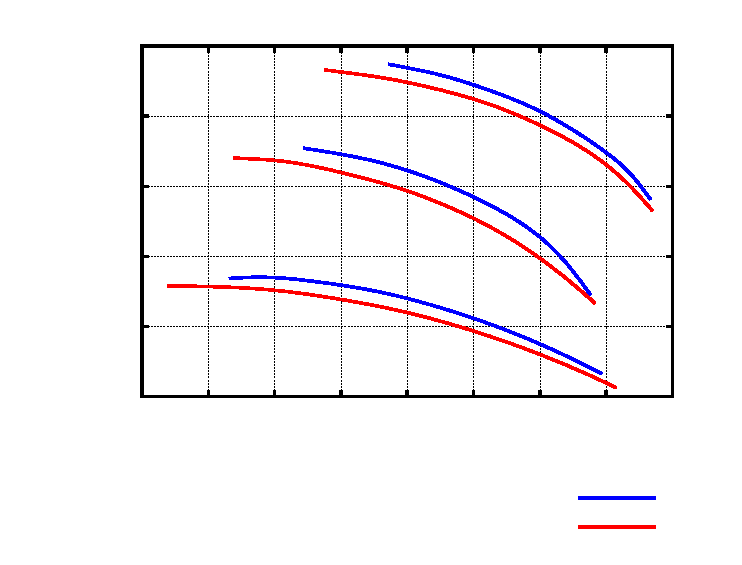
\includegraphics[width={340.10bp},height={255.10bp}]{teresch1988turb}}%
    \gplfronttext
  \end{picture}%
\endgroup

	}
	\caption{Характеристика ступени осевого компрессора с турбулизаторами на входном участке лопаток рабочего колеса \cite{Tereschenko1988}}
	\label{fig:Tereschenko1988turb}
\end{figure}

Применение многорядных решёток лопаток \cite{Tereschenko2015,Qiushi2010,LIU2022,Bammert1980,McGlumphy2009,VanEck2023,Wennerstrom1990} выглядит перспективным для применения в вентиляторных и компрессорных ступенях, так как характеристики подобных плоских решёток свидетельствуют о возможности получения большего поворота потока при меньших потерях полного давления. 

Экспериментальное исследование модели относительно высоконагруженной ступени (расчётный \(\Ht\) равен 0,45) \cite{LIU2022} продемонстрировали преимущество ступеней с двухрядными венцами РК и СА перед ступенями с однорядными венцами при расходе меньшем расчётного. Ступень из двухрядных решёток имела больший запас до срыва (рисунок \ref{fig:LIU2022}). Однако измеренный КПД на расчётном режиме оказался всего на 0,6\% выше чем у исходной ступени.
\begin{figure}[ht]
	\centerfloat{
% GNUPLOT: LaTeX picture with Postscript
\begingroup
  \makeatletter
  \providecommand\color[2][]{%
    \GenericError{(gnuplot) \space\space\space\@spaces}{%
      Package color not loaded in conjunction with
      terminal option `colourtext'%
    }{See the gnuplot documentation for explanation.%
    }{Either use 'blacktext' in gnuplot or load the package
      color.sty in LaTeX.}%
    \renewcommand\color[2][]{}%
  }%
  \providecommand\includegraphics[2][]{%
    \GenericError{(gnuplot) \space\space\space\@spaces}{%
      Package graphicx or graphics not loaded%
    }{See the gnuplot documentation for explanation.%
    }{The gnuplot epslatex terminal needs graphicx.sty or graphics.sty.}%
    \renewcommand\includegraphics[2][]{}%
  }%
  \providecommand\rotatebox[2]{#2}%
  \@ifundefined{ifGPcolor}{%
    \newif\ifGPcolor
    \GPcolorfalse
  }{}%
  \@ifundefined{ifGPblacktext}{%
    \newif\ifGPblacktext
    \GPblacktexttrue
  }{}%
  % define a \g@addto@macro without @ in the name:
  \let\gplgaddtomacro\g@addto@macro
  % define empty templates for all commands taking text:
  \gdef\gplbacktext{}%
  \gdef\gplfronttext{}%
  \makeatother
  \ifGPblacktext
    % no textcolor at all
    \def\colorrgb#1{}%
    \def\colorgray#1{}%
  \else
    % gray or color?
    \ifGPcolor
      \def\colorrgb#1{\color[rgb]{#1}}%
      \def\colorgray#1{\color[gray]{#1}}%
      \expandafter\def\csname LTw\endcsname{\color{white}}%
      \expandafter\def\csname LTb\endcsname{\color{black}}%
      \expandafter\def\csname LTa\endcsname{\color{black}}%
      \expandafter\def\csname LT0\endcsname{\color[rgb]{1,0,0}}%
      \expandafter\def\csname LT1\endcsname{\color[rgb]{0,1,0}}%
      \expandafter\def\csname LT2\endcsname{\color[rgb]{0,0,1}}%
      \expandafter\def\csname LT3\endcsname{\color[rgb]{1,0,1}}%
      \expandafter\def\csname LT4\endcsname{\color[rgb]{0,1,1}}%
      \expandafter\def\csname LT5\endcsname{\color[rgb]{1,1,0}}%
      \expandafter\def\csname LT6\endcsname{\color[rgb]{0,0,0}}%
      \expandafter\def\csname LT7\endcsname{\color[rgb]{1,0.3,0}}%
      \expandafter\def\csname LT8\endcsname{\color[rgb]{0.5,0.5,0.5}}%
    \else
      % gray
      \def\colorrgb#1{\color{black}}%
      \def\colorgray#1{\color[gray]{#1}}%
      \expandafter\def\csname LTw\endcsname{\color{white}}%
      \expandafter\def\csname LTb\endcsname{\color{black}}%
      \expandafter\def\csname LTa\endcsname{\color{black}}%
      \expandafter\def\csname LT0\endcsname{\color{black}}%
      \expandafter\def\csname LT1\endcsname{\color{black}}%
      \expandafter\def\csname LT2\endcsname{\color{black}}%
      \expandafter\def\csname LT3\endcsname{\color{black}}%
      \expandafter\def\csname LT4\endcsname{\color{black}}%
      \expandafter\def\csname LT5\endcsname{\color{black}}%
      \expandafter\def\csname LT6\endcsname{\color{black}}%
      \expandafter\def\csname LT7\endcsname{\color{black}}%
      \expandafter\def\csname LT8\endcsname{\color{black}}%
    \fi
  \fi
    \setlength{\unitlength}{0.0500bp}%
    \ifx\gptboxheight\undefined%
      \newlength{\gptboxheight}%
      \newlength{\gptboxwidth}%
      \newsavebox{\gptboxtext}%
    \fi%
    \setlength{\fboxrule}{0.5pt}%
    \setlength{\fboxsep}{1pt}%
    \definecolor{tbcol}{rgb}{1,1,1}%
\begin{picture}(6802.00,5102.00)%
    \gplgaddtomacro\gplbacktext{%
      \csname LTb\endcsname%%
      \put(1204,2016){\makebox(0,0)[r]{\strut{}$0,35$}}%
      \csname LTb\endcsname%%
      \put(1204,2717){\makebox(0,0)[r]{\strut{}$0,4$}}%
      \csname LTb\endcsname%%
      \put(1204,3419){\makebox(0,0)[r]{\strut{}$0,45$}}%
      \csname LTb\endcsname%%
      \put(1204,4120){\makebox(0,0)[r]{\strut{}$0,5$}}%
      \csname LTb\endcsname%%
      \put(1204,4821){\makebox(0,0)[r]{\strut{}$0,55$}}%
      \csname LTb\endcsname%%
      \put(1372,1736){\makebox(0,0){\strut{}$0,4$}}%
      \csname LTb\endcsname%%
      \put(1978,1736){\makebox(0,0){\strut{}$0,45$}}%
      \csname LTb\endcsname%%
      \put(2584,1736){\makebox(0,0){\strut{}$0,5$}}%
      \csname LTb\endcsname%%
      \put(3191,1736){\makebox(0,0){\strut{}$0,55$}}%
      \csname LTb\endcsname%%
      \put(3797,1736){\makebox(0,0){\strut{}$0,6$}}%
      \csname LTb\endcsname%%
      \put(4403,1736){\makebox(0,0){\strut{}$0,65$}}%
      \csname LTb\endcsname%%
      \put(5009,1736){\makebox(0,0){\strut{}$0,7$}}%
      \put(5177,2016){\makebox(0,0)[l]{\strut{}$0,75$}}%
      \put(5177,2717){\makebox(0,0)[l]{\strut{}$0,8$}}%
      \put(5177,3419){\makebox(0,0)[l]{\strut{}$0,85$}}%
      \put(5177,4120){\makebox(0,0)[l]{\strut{}$0,9$}}%
      \put(5177,4821){\makebox(0,0)[l]{\strut{}$0,95$}}%
    }%
    \gplgaddtomacro\gplfronttext{%
      \csname LTb\endcsname%%
      \put(266,3418){\rotatebox{-270}{\makebox(0,0){\strut{}$\Ht$}}}%
      \put(6157,3418){\rotatebox{-270}{\makebox(0,0){\strut{}$\eta$}}}%
      \put(3190,1316){\makebox(0,0){\strut{}$\ca$}}%
      \csname LTb\endcsname%%
      \put(3938,1043){\makebox(0,0)[r]{\strut{}$\Ht$ двухрядный}}%
      \csname LTb\endcsname%%
      \put(3938,763){\makebox(0,0)[r]{\strut{}$\Ht$ однорядный}}%
      \csname LTb\endcsname%%
      \put(3938,483){\makebox(0,0)[r]{\strut{}$\eta$ двухрядный}}%
      \csname LTb\endcsname%%
      \put(3938,203){\makebox(0,0)[r]{\strut{}$\eta$ однорядный}}%
    }%
    \gplbacktext
    \put(0,0){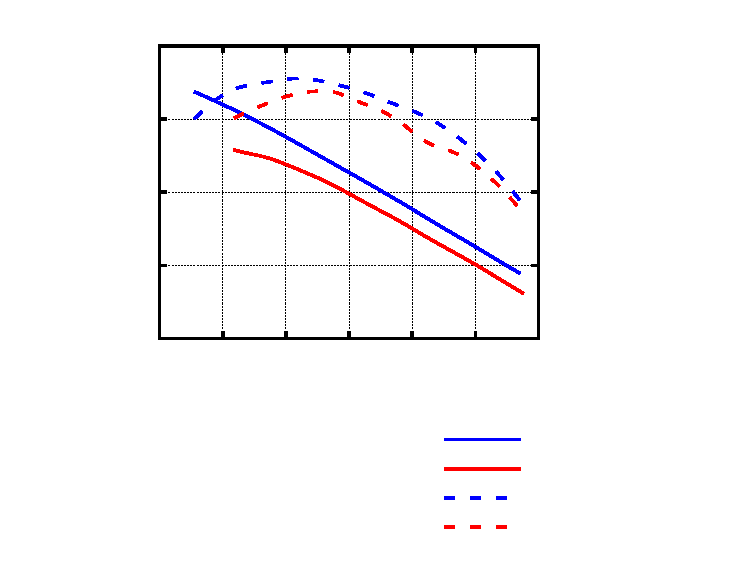
\includegraphics[width={340.10bp},height={255.10bp}]{LIU2022}}%
    \gplfronttext
  \end{picture}%
\endgroup

	}
	\caption{Сравнение характеристик ступени с двухрядными и однорядными венцами \cite{LIU2022}}
	\label{fig:LIU2022}
\end{figure}

Градиент давления при течении в проточной части можно скомпенсировать, плавно увеличивая скорости потока вдоль течения, за счет уменьшения сечения проточной части от входа к выходу из вентилятора. Такие вентиляторы называются вентиляторами с меридиональным ускорением потока. Уменьшение сечения проточной части, как правило, обеспечивается плавным увеличением относительного диаметра втулки \(\bar{d}\) (рисунок \ref{fig:schemaMrdnl}). Характеристикой течения в проточной части с меридиональным ускорением потока является отношение осевых плотностей тока на входе (1) и выходе (2) из решётки (Axial velocity density ratio) \(AVDR = \rho_2 C_\text{2a}/\rho_1 C_\text{1a}\). Для несжимаемого газа, соответственно, коэффициент меридионального ускорения \(m = C_\text{2a}/C_\text{1a}\). 
\begin{figure}[ht]
	\centerfloat{
		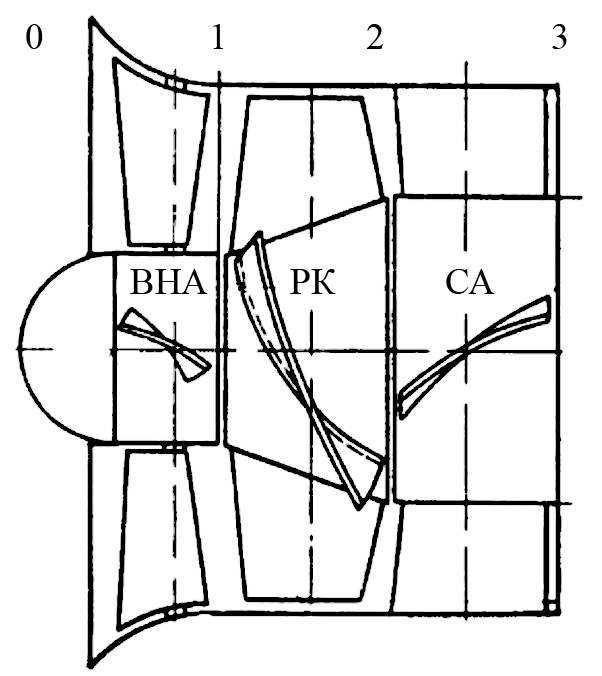
\includegraphics[width=8cm,keepaspectratio]{images/schemaMrdnl}
	}
	\caption{Схема вентилятора с меридиональным ускорением потока \cite{Brusilovskiy2004}}
	\label{fig:schemaMrdnl}
\end{figure}

При отношении осевых скоростей при входе и выходе из решётки больше 1, то есть при ускорении потока, пограничные слои на элементах проточной части вентилятора должны становиться тоньше, отрыв потока должен затягиваться, а потери полного давления снижаться. По результатам работы \cite{SenthilKumaran2015} по исследованию влияния \(AVDR\) на характеристики компрессорной ступени было установлено, что увеличение \(AVDR\) способствует росту КПД ступени до некоторого предельного значения, после которого увеличение \(AVDR\) уже не приводит к заметным изменениям. 
 
Снижение диффузорности течения позволяет получить эффективные вентиляторы в области параметров, выходящей за границы значений параметров типичных для эффективной осевой ступени с цилиндрической проточной частью \cite{Eck1972}. Спроектированный на сравнительно большое значение коэффициента теоретического напора \(\Ht\) равном 0,52 при коэффициенте расхода в сечении за рабочим колесом \(\bar{c}_\text{2a}\) равном 0,55 вентилятор \cite{Brusilovskiy1962} показал достаточно высокий КПД равный 0,865 и хорошее регулирование поворотом лопаток входного направляющего аппарата. Максимальное значение приведённого напора \(\bar{H}\) при регулировании составило примерно 0,6. Меридиональное ускорение потока происходило по большей части в рабочем колесе, где относительный диаметр втулки \(\bar{d}\)  менялся от 0,545 перед рабочим колесом до 0,7 перед спрямляющим аппаратом. Спрямляющий аппарат был выполнен с цилиндрической проточной частью. Степень реактивности на среднем радиусе составила 0,74.

Большое экспериментальное исследование вентиляторов с меридиональным ускорением потока предназначенных для местного проветривания в шахтах было проведено С.~К.~Ивановым \cite{Ivanov1969}. В результате исследований были спроектированы схемы вентиляторов с меридиональным ускорением потока в рабочем колесе, подходящие по требованиям для местного проветривания шахт. Они сочетают уровень коэффициента напора \(\bar{H}\) от 0,35 до 0,4 при коэффициентах расхода \(\bar{c}_\text{2a}\) от 0,4 до 0,6, максимальные КПД \(\eta\) от 0,85 до 0,87, при этом обладая хорошей регулируемостью поворотом входного направляющего аппарата.

Большие значения \(\Ht\) ступеней характерны для авиационных двигателей. Уменьшение удельного веса и повышение количества полезной подведённой энергии критичны для авиационной техники в целом. В вентиляторных ступенях авиационных газотурбинных двигателей (ГТД) в связи с относительно малой величиной втулки \(\bar{d}\) и высоким коэффициентом напора \(\bar{H}\) велик риск наступления срыва потока \cite{Kazandjan1983}. Для предотвращения срыва потока и повышения напора обеспечивается ускорение осевой компоненты скорости в межлопаточных каналах.

%Развитие рынка микро-ГТД интенсифицирует развитие диагональных ступеней компрессоров \cite{Cevik2009, Kock2017,VanEck2023}, во многом близких к осевым вентиляторам с меридиональным ускорением потока. Такие ступени применительно в микро-ГТД имеют меньшие радиальные габариты чем центробежные ступени и развивают больший коэффициент напора \(\bar{H}\) чем осевые ступени.

\section{Профилирование лопаток вентилятора с меридиональным ускорением}

Работа подводимая к рабочему телу в рабочем колесе \(H_\text{т}\), \(\si\joule/\si\kilogram\), турбомашины определяется кинематикой потока через уравнение Эйлера:
\begin{equation}
	H_\text{т} = U_2 C_{2u} - U_2 C_{1u},
	\label{eq:Ht}
\end{equation}
или в безразмерном виде (параграф \ref{sec:ch1/sec1}):
\begin{equation}
	\bar{H}_\text{т} = H_\text{т}/U_\text{к}^2 = \bar{r}_2 \bar{c}_{2u} - \bar{r}_1 \bar{c}_{1u},
	\label{eq:H_t}
\end{equation}
\begin{eqexpl}
	\item{\(U\)} окружная скорость колеса, \(\si\meter/\si\second\);
	\item{\(U_\text{к}\)} окружная скорость периферии колеса, \(\si\meter/\si\second\);
	\item{\(C_{u}\)} окружная компонента скорости потока, \(\si\meter/\si\second\);
	\item{\(\bar{c}_{u}\)} коэффициент окружной компоненты скорости потока, \(C_{u}/U\);
	\item{\(\bar{r}\)} приведённый радиус, \(r/R\);
	\item{\(R\)} радиус рабочего колеса, \(\si\meter\).
\end{eqexpl}
Задаваясь необходимым коэффициентом расхода \(\bar{c}_\text{a}\) коэффициент теоретического напора определяется только направлениями скоростей перед и за колесом:
\begin{equation}
	\bar{H}_\text{т} = \bar{r}_2 \bar{c}_\text{2a} \tan\alpha_2 - \bar{r}_1 \bar{c}_{1a} \tan\alpha_1,
	\label{eq:H_t_tan}
\end{equation}

Профилирование лопаток турбомашины подразумевает формирование геометрии лопаточных венцов, обеспечивающей необходимую кинематику потока, то есть обеспечение заданных направлений скоростей, давления и расхода. 

Течение в лопаточном венце сложно для описания –-- вторичные течения, нестационарность течения, взаимодействия пограничных слоёв на поверхностях лопаток и периферийных поверхностях, теплообмен, вибрация лопаток и т.д. При проектировании обычно используют математические модели, в значительной мере упрощающие действительное течение, начиная с того, что  считают течение установившимся.

\subsection{Профилирование лопаток цилиндрической ступени}\label{sec:ch1/profil}

 Традиционным упрощением при рассмотрении течения в осевой ступени является гипотеза плоских сечений, впервые высказанная Н.Е. Жуковским \cite{Joukovskiy1949}. Согласно этой гипотезе течение в проточной части можно разделить коаксиальными поверхностями на элементарные цилиндрические слои течения. При этом течения в соседних слоях в первом приближении независимы. Уравнение \ref{eq:H_t_tan} преобразуется к виду:
\begin{equation}
	\bar{H}_\text{т} = \bar{c}_\text{a} \left( \tan\alpha_2 - \tan\alpha_1 \right).
	\label{eq:H_t_cil}
\end{equation}
\begin{eqexpl}
	\item{$\alpha$} угол между скоростью потока в абсолютном движении и осью решётки.
\end{eqexpl}

Далее, каждый элементарный цилиндрический слой течения разворачивается на плоскость, образуя бесконечную решётку профилей. Рассматривая течение в этой плоскости в относительном движении, то есть в системе координат, в которой решётка остаётся неподвижной, разница в окружных компонентах скорости остаётся той же, что и в абсолютной системе координат: \(\Delta C_\text{u} = \Delta W_\text{u}\), соответственно \(\tan\alpha_2 - \tan\alpha_1 = \tan\beta_2 - \tan\beta_1\), где \(\beta\) "--- угол направления скорости в относительном движении. Течение газа в неподвижной плоской решётке профилей и определение величины \(\tan\beta_2 - \tan\beta_1\) сравнительно просто поддаётся теоретическому и экспериментальному исследованию. 

Данный подход, основанный на идеализированном двухмерном потоке, позволяет строить действующие машины с эксплуатационными параметрами близкими к расчётным. Гипотеза плоских сечений отражает основную суть явлений при обтекании лопаточных венцов турбомашин. Учёт остальных явлений проводится в процессе уточнения основного решения полученного на основе рассмотрения двухмерного течения в решётках профилей.

Для описания геометрии решёток и профиля используются следующие параметры (рисунок \ref{fig:cascad}).  
\begin{figure} [ht]
	\centerfloat{
		\includegraphics{images/cascad}
	}
	\caption{Основные геометрические параметры профиля и решётки профилей} 
	\label{fig:cascad}
\end{figure}
\eqexplSetIntro{}
\begin{eqexpl}
\item{\(c\)}  толщина профиля, максимальное расстояние между ближайшими точками корытца и спинки, \(\si\meter\); 
\item{\(b\)} хорда профиля, расстояние между крайними точками средней линии профиля, \(\si\meter\); 
\item{\(f\)} изгиб профиля, максимальное расстояние от средней линии до хорды профиля, \(\si\meter\);
\item{\(t\)} шаг решётки, расстояние между соответствующими точками соседних профилей, \(\si\meter\).
%\item{средняя линия профиля} геометрическое множество точек, не выходящее за контур профиля, минимальное расстояние от которых одинаково до линий корытца и спинки профиля.
\end{eqexpl}

Для характеристики профиля в решётке будем использовать относительные величины: 
\begin{eqexpl}
\item{\(\bar{c}\)} относительная толщина профиля, \(c/b\); 
\item{\(\bar{f}\)} относительный изгиб профиля, \(f/b\);
\item{\(\tau\)} густота решётки, \(b/t\).
\end{eqexpl}

Линия соединяющая соответствующие точки профилей называется фронтом решётки, а нормальная к ней – осью решётки. Углы, характеризующие расположение профилей в решётке, обозначаются следующим образом:
\begin{eqexpl}
\item{\(\theta_{\text{г}}\)} угол установки, угол между осью решетки и хордой профиля; 
\item{\(\beta_\text{л}\)} углы между касательными к средней линии профиля и осью решётки в точках передней (1) и задней кромки (2);
\item{\(\upsilon\)} угол изгиба профиля.
\end{eqexpl}
\eqexplSetIntro{где}

Задача определения геометрии решётки, обеспечивающей необходимую кинематику потока, является обратной задачей аэродинамики. Количество неизвестных в этой задаче меньше количества параметров, и заданную кинематику может обеспечить бесконечное число вариантов решёток профилей. Для невязкого несжимаемого течения угол атаки \(i\) и изгиб профиля \(\bar{f}\) являются практически эквивалентными способами обеспечить необходимую кинематику потока "--- для каждого \(i\) можно подобрать такой \(\bar{f}\), что будет обеспечен необходимый поворот потока. Однако в случае вязкого течения меньшие потери полного давления соответствуют течению в решётках с небольшими углами атаки. Все эти решётки будут отличаться по своим эксплуатационным характеристикам, таким как прочность, эффективность, диапазон эффективной работы. Для замыкания задачи профилирования задаются углом атаки \(i\) и густотой решётки \(\tau\), исходя из опыта проектирования машин различного назначения.

Авторы исследований по разному определяют значения номинального угла атаки, характеризуемого режимом работы решётки. Хауэлл \cite{Howell1945} считал, что угол атаки должен лежать в пределах от минус 5 до плюс 5 градусов. Либляйн \cite{Lieblein1959} принимал за номинальный угол атаки соответствующий минимуму потерь полного давления в решётке. 

А.\,П.\,Комаров \cite{Komarov1967} определил номинальный угол атаки, как соответствующий максимальному КПД решётки. На основании обработки большого количества экспериментальных продувок решёток профилей им была предложена приближенная формула для нахождения угла атаки, соответствующего максимальному КПД решётки:
\begin{equation}
	i_{\eta_\text{max}}=4,5-0,3\frac{\upsilon}{\tau} \left[ 1,81- \left(2\bar{x}_{f}\right)^2 \right],
\end{equation}
\begin{eqexpl}
	\item{\(\upsilon\)} угол изгиба профиля, \(\si\degree\);
	\item{\(\bar{x}_f\)} относительное положение точки средней линии профиля с максимальным изгибом;
\end{eqexpl}

В работе \cite{Emery1951} номинальным углом атаки принят тот при котором реализуется плавное распределение профиля давления на контуре лопатки. Угол атаки соответствующий безударному входу, при котором точка торможения потока располагается на передней кромке был принят в качестве номинального в работе \cite{Judin1947}. В работе \cite{Brusilovskiy1986}, для учета действия центробежных сил на течение во вращающихся решётках профилей, рекомендуется для периферии рабочего колеса вентилятора выбирать  небольшие отрицательные величины углов атаки от минус 2 до минус 3, а для привтулочных сечений от плюс 2 до плюс 4.

Работа совершённая над рабочем телом рабочим колесом должна быть достаточна для работы при меньших скоростях в целях обеспечения необходимой механического прочности лопаточного венца и снижения уровня шума, но, при этом, аэродинамическая нагруженность недостаточна для образования отрыва потока и работе с низкой эффективностью. Аэродинамическая нагруженность при небольших углах атаки \(i\) в большой степени зависит от густоты решётки \(\tau\). Подход к выбору рационального значения \(\tau\) во многих исследованиях различен. С.\,А.\,Довжик \cite{Dovjik1968} при значениях коэффициента теоретической работы \(\Ht\) не более 0,3, исходя из опыта проектирования компрессоров, рекомендует значения \(\tau\) на среднем радиусе от 1,0 до 1,2. Хауэлл \cite{Howell1945} для своего номинального режима работы рекомендует для определения рационального значения \(\tau\) зависимость от направления потока показанную на рисунке \ref{fig:tauRek}. В работе \cite{Bunimovich1967} А.\,И.\,Бунимовичем и А.\,А.\,Святогоровым проведено экспериментальное исследование характеристик плоских компрессорных решёток профилей и обобщение его результатов. Одним из результатов работы стали рекомендации по выбору оптимальной густоты решётки (рисунок \ref{fig:tauRek}). Для концевых сечений рекомендуемые густоты и углы атаки отличаются от выбранных по продувкам плоских решёток \cite{Brusilovskiy1975b}.
\begin{figure} [ht]
	\centerfloat{
		% GNUPLOT: LaTeX picture with Postscript
\begingroup
  \makeatletter
  \providecommand\color[2][]{%
    \GenericError{(gnuplot) \space\space\space\@spaces}{%
      Package color not loaded in conjunction with
      terminal option `colourtext'%
    }{See the gnuplot documentation for explanation.%
    }{Either use 'blacktext' in gnuplot or load the package
      color.sty in LaTeX.}%
    \renewcommand\color[2][]{}%
  }%
  \providecommand\includegraphics[2][]{%
    \GenericError{(gnuplot) \space\space\space\@spaces}{%
      Package graphicx or graphics not loaded%
    }{See the gnuplot documentation for explanation.%
    }{The gnuplot epslatex terminal needs graphicx.sty or graphics.sty.}%
    \renewcommand\includegraphics[2][]{}%
  }%
  \providecommand\rotatebox[2]{#2}%
  \@ifundefined{ifGPcolor}{%
    \newif\ifGPcolor
    \GPcolorfalse
  }{}%
  \@ifundefined{ifGPblacktext}{%
    \newif\ifGPblacktext
    \GPblacktexttrue
  }{}%
  % define a \g@addto@macro without @ in the name:
  \let\gplgaddtomacro\g@addto@macro
  % define empty templates for all commands taking text:
  \gdef\gplbacktext{}%
  \gdef\gplfronttext{}%
  \makeatother
  \ifGPblacktext
    % no textcolor at all
    \def\colorrgb#1{}%
    \def\colorgray#1{}%
  \else
    % gray or color?
    \ifGPcolor
      \def\colorrgb#1{\color[rgb]{#1}}%
      \def\colorgray#1{\color[gray]{#1}}%
      \expandafter\def\csname LTw\endcsname{\color{white}}%
      \expandafter\def\csname LTb\endcsname{\color{black}}%
      \expandafter\def\csname LTa\endcsname{\color{black}}%
      \expandafter\def\csname LT0\endcsname{\color[rgb]{1,0,0}}%
      \expandafter\def\csname LT1\endcsname{\color[rgb]{0,1,0}}%
      \expandafter\def\csname LT2\endcsname{\color[rgb]{0,0,1}}%
      \expandafter\def\csname LT3\endcsname{\color[rgb]{1,0,1}}%
      \expandafter\def\csname LT4\endcsname{\color[rgb]{0,1,1}}%
      \expandafter\def\csname LT5\endcsname{\color[rgb]{1,1,0}}%
      \expandafter\def\csname LT6\endcsname{\color[rgb]{0,0,0}}%
      \expandafter\def\csname LT7\endcsname{\color[rgb]{1,0.3,0}}%
      \expandafter\def\csname LT8\endcsname{\color[rgb]{0.5,0.5,0.5}}%
    \else
      % gray
      \def\colorrgb#1{\color{black}}%
      \def\colorgray#1{\color[gray]{#1}}%
      \expandafter\def\csname LTw\endcsname{\color{white}}%
      \expandafter\def\csname LTb\endcsname{\color{black}}%
      \expandafter\def\csname LTa\endcsname{\color{black}}%
      \expandafter\def\csname LT0\endcsname{\color{black}}%
      \expandafter\def\csname LT1\endcsname{\color{black}}%
      \expandafter\def\csname LT2\endcsname{\color{black}}%
      \expandafter\def\csname LT3\endcsname{\color{black}}%
      \expandafter\def\csname LT4\endcsname{\color{black}}%
      \expandafter\def\csname LT5\endcsname{\color{black}}%
      \expandafter\def\csname LT6\endcsname{\color{black}}%
      \expandafter\def\csname LT7\endcsname{\color{black}}%
      \expandafter\def\csname LT8\endcsname{\color{black}}%
    \fi
  \fi
    \setlength{\unitlength}{0.0500bp}%
    \ifx\gptboxheight\undefined%
      \newlength{\gptboxheight}%
      \newlength{\gptboxwidth}%
      \newsavebox{\gptboxtext}%
    \fi%
    \setlength{\fboxrule}{0.5pt}%
    \setlength{\fboxsep}{1pt}%
    \definecolor{tbcol}{rgb}{1,1,1}%
\begin{picture}(9070.00,6802.00)%
    \gplgaddtomacro\gplbacktext{%
      \csname LTb\endcsname%%
      \put(868,1456){\makebox(0,0)[r]{\strut{}$0$}}%
      \csname LTb\endcsname%%
      \put(868,2089){\makebox(0,0)[r]{\strut{}$10$}}%
      \csname LTb\endcsname%%
      \put(868,2722){\makebox(0,0)[r]{\strut{}$20$}}%
      \csname LTb\endcsname%%
      \put(868,3355){\makebox(0,0)[r]{\strut{}$30$}}%
      \csname LTb\endcsname%%
      \put(868,3989){\makebox(0,0)[r]{\strut{}$40$}}%
      \csname LTb\endcsname%%
      \put(868,4622){\makebox(0,0)[r]{\strut{}$50$}}%
      \csname LTb\endcsname%%
      \put(868,5255){\makebox(0,0)[r]{\strut{}$60$}}%
      \csname LTb\endcsname%%
      \put(868,5888){\makebox(0,0)[r]{\strut{}$70$}}%
      \csname LTb\endcsname%%
      \put(868,6521){\makebox(0,0)[r]{\strut{}$80$}}%
      \csname LTb\endcsname%%
      \put(1789,1176){\makebox(0,0){\strut{}$-20$}}%
      \csname LTb\endcsname%%
      \put(3295,1176){\makebox(0,0){\strut{}$0$}}%
      \csname LTb\endcsname%%
      \put(4801,1176){\makebox(0,0){\strut{}$20$}}%
      \csname LTb\endcsname%%
      \put(6306,1176){\makebox(0,0){\strut{}$40$}}%
      \csname LTb\endcsname%%
      \put(7812,1176){\makebox(0,0){\strut{}$60$}}%
    }%
    \gplgaddtomacro\gplfronttext{%
      \csname LTb\endcsname%%
      \put(266,3988){\rotatebox{-270}{\makebox(0,0){\strut{}$\Delta\beta, \si\degree$}}}%
      \put(4800,756){\makebox(0,0){\strut{}$\beta_2, \si\degree$}}%
      \csname LTb\endcsname%%
      \put(7494,483){\makebox(0,0)[r]{\strut{}Бунимович, Святогоров \cite{Bunimovich1967}}}%
      \csname LTb\endcsname%%
      \put(7494,203){\makebox(0,0)[r]{\strut{}Хауэлл \cite{Howell1945}}}%
    }%
    \gplbacktext
    \put(0,0){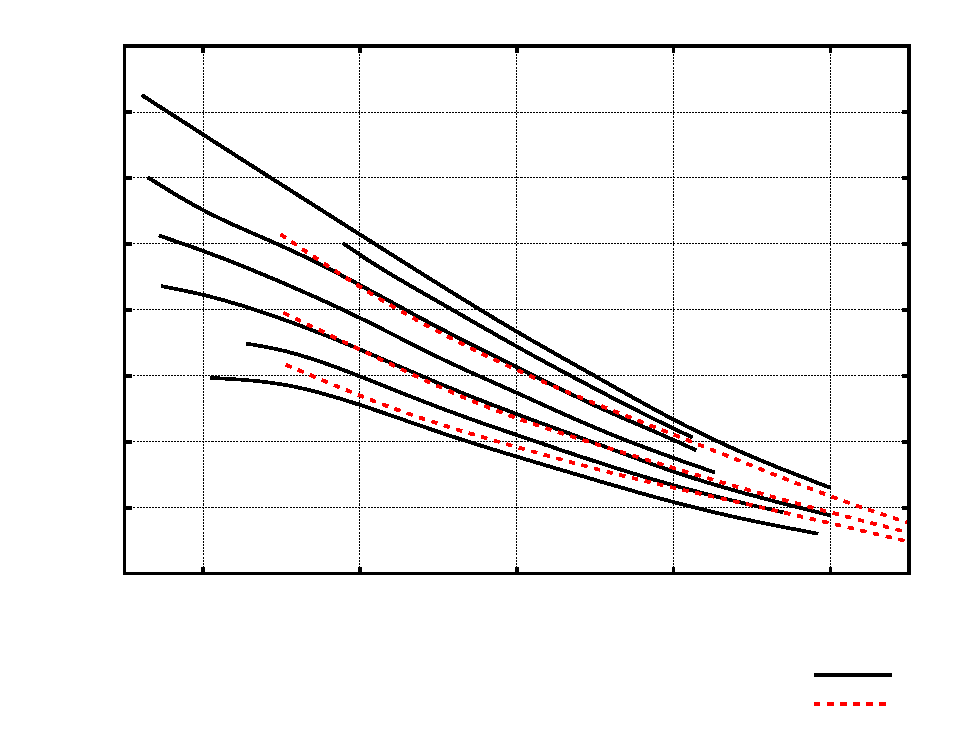
\includegraphics[width={453.50bp},height={340.10bp}]{BunSvjat}}%
    \gplfronttext
  \end{picture}%
\endgroup

	}
	\caption{Рекомендуемые значения густоты решётки \(\tau\) в зависимости от угла потока на выходе из решётки \(\beta_2\) и углом поворота потока \(\Delta\beta\)} 
	\label{fig:tauRek}
\end{figure}

После того как угол атаки \(i\) и густота решётки \(\tau\) определены, остаётся определить необходимый изгиб профиля \(\bar{f}\). Значение \(\bar{f}\) определяется либо из результатов обобщения экспериментальных продувок \cite{Emery1951,Bunimovich1967}, либо на основе теоретических характеристик \cite{Umnov1951,Uschakov1960,Bloch1961}, полученных при рассмотрении потенциального течения. 

Связь между направлением идеального потока перед и за решёткой профилей выражаются в виде зависимости \( \tan\beta_2 = A\tan\beta_1+B\), где \(A\) и \(B\) "--- коэффициенты характеризуемые геометрией решётки. Для определения \(A\) и \(B\) используются метод отображения \cite{Bloch1961}, или метод наложения потоков. В методе отображения используется течение в области которое можно посчитать. Течение в исследуемой области может быть изучено с помощью конформного преобразования. При использовании метода наложения потоков на контуре профиля располагается большое количество особенностей: вихрей, источников или диполей. Задача об определении характеристик решётки сводится к решению системы линейных алгебраических уравнений. 

Широкое распространение получил метод дискретных вихрей (МДВ) \cite{Belozerovskiy1978}. Бесконечная решётка профилей обтекается потенциальным невязким несжимаемым потоком. На контуре профиля расставляются точки дискретных вихрей и контрольные точки (рисунок \ref{fig:foilVortex}). В контрольных точках принимается, что поток касателен к контуру профиля. Необходимо задать критическую точку схода потока с профиля, в которой интенсивность вихря будет нулевой. На остальных профилях решётки вихри располагаются точно так же, как и на исходном профиле, образуя бесконечные цепочки вихрей. 

\begin{figure} [ht]
	\centerfloat{
		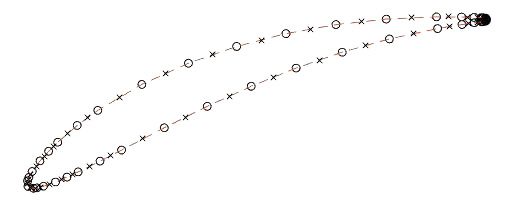
\includegraphics[width=8cm,keepaspectratio]{images/foilVortex} 
	} 
	\caption{Вихри \(\times\) и контрольные точки \(\circ\) на контуре профиля} 
	\label{fig:foilVortex}
\end{figure}

\subsection{Течение в вентиляторе с меридиональным ускорением}\label{sec:ch1/mrdnl}

При исследовании цилиндрических ступеней за прошедшее время было накоплено огромное количество экспериментальных данных и отработано большое число математических моделей. При любых изменениях в характере течения следует максимально полно использовать существующие модели и дополнять их по мере необходимости. Для моделирования течения и проектирования вентилятора с меридиональным ускорением потока, за основу берутся показавшие хорошие результаты модели течения в цилиндрической ступени.

Теория течения в меридиональном сечении развита в работах Ву \cite{Wu1952}, который предложил в качестве условных поверхностей тока поверхности \(S_1\) и \(S_2\) (рисунок \ref{fig:s1s2}). В качестве поверхности \(S_1\) принята традиционная поверхность от лопатки к лопатке. Поверхности тока \(S_2\) имеют радиальную форму перед лопатками, а в межлопаточном канале они изгибаются и скручиваются.

\begin{figure} [ht]
	\centerfloat{
		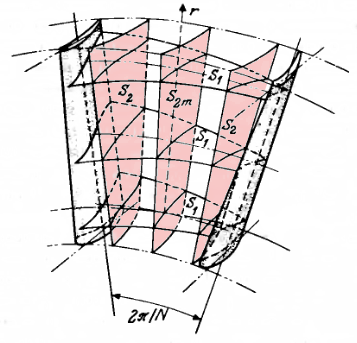
\includegraphics[width=8cm,keepaspectratio]{images/s1s2}
	}
	\caption{Поверхности тока \(S_1\) и \(S_2\) \cite{Wu1952}. \(S_2\) выделены красным} 
	\label{fig:s1s2}
\end{figure}

Следуя гипотезе плоских сечений, обычно пренебрегают скручиванием поверхностей \(S_1\). Их рассматривают, как образованные вращением от кривых линий тока в меридиональной плоскости вокруг оси турбомашины \cite{Sirotkin1972}. Параметры течения в межвенцовом зазоре определяются по углам наклона меридиональных линий и закону закрутки рабочего тела из уравнения радиального равновесия \cite{Smith1966} с помощью численных методов.

В осевых ступенях с умеренным отклонением поверхностей тока \(S_1\) от цилиндричности, не превышающей 15 градусов, используются методы теоретического анализа течения в лопаточных венцах для осевых турбомашин с цилиндрической проточной частью \cite{Sirotkin1972,Stepanov1962}, влиянием радиальной компоненты скорости при этом пренебрегают. 

Схема вентилятора с меридиональным ускорением подразумевает значительное увеличение коэффициента расхода в одной ступени и изменение радиуса линий тока в сечениях у втулки. Течение в таком лопаточном венце имеет выраженный трехмерный характер, определяемый значительной величиной радиальной составляющей скорости. Рассматривая невязкое безвихревое течение несжимаемого газа в решётке профилей на поверхностях \(S_1\), с помощью конформного отображения можно перейти к рассмотрению обтекания плоской решётки профилей в слое переменной толщины. 

При предварительном проектировании многоступенчатого компрессора, пользуются развёрткой на плоскость усечённого конуса (плоскость~\(W\))~\cite{Sachkova2000}: 
\begin{equation}
	W = r e^{i\varphi},
\end{equation}
\begin{eqexpl}
	\item{\(r, \phi\)} полярные координаты.
\end{eqexpl}

Отображение плоскости \(W\) на плоскость \(z\) с декартовыми координатами \(x\) и \(y\) проводится при помощи логарифмической функции 
\begin{equation}
z = \ln W,
\end{equation}
тогда координаты связанны выражениями:
\begin{equation}
	x = \ln r, y = \varphi.
\end{equation}

 В работе \cite{Nikitin1966} экспериментально изучено течение в диагональных решётках профилей, полученных таким отображением. Полученные характеристики  показали хорошее совпадение по величине отклонения потока в сравнении с исходной плоской решёткой профилей при безотрывном течении и различных числах Маха на входе в решётку \(M_1\) от 0,3 до 0,65. Использование продувок плоских профилей для определения характеристик диагональных решёток имеет недостаток "--- течение в пограничном слое вихревое и не переносится на исследуемую плоскость при конформных отображениях. Отображением можно пользоваться только при безотрывном течении и достаточно тонких пограничных слоях. На рисунке \ref{fig:nikitin} приводится сравнение распределения относительных  скоростей \(\bar{w} = w/W_1\) (где \(w\) "--- скорость на спинке, м/с; \(W_1\) "--- скорость перед решёткой, м/с)  на спинке лопатки, полученных экспериментально и пересчётом продувки соответствующей плоской решётки. Сравнение выполнено при трёх различных углах атаки и \(M_1\) приблизительно равном 0,5. При небольших отрицательных углах атаки имеет место хорошее совпадение, а по мере роста толщины пограничного слоя при увеличении угла атаки, отличия становятся существенными.
 
 \begin{figure} [ht]
 	\centerfloat{
 		%\includegraphics[width=8cm,keepaspectratio]{images/nikitin1966}
 		% GNUPLOT: LaTeX picture with Postscript
\begingroup
  \makeatletter
  \providecommand\color[2][]{%
    \GenericError{(gnuplot) \space\space\space\@spaces}{%
      Package color not loaded in conjunction with
      terminal option `colourtext'%
    }{See the gnuplot documentation for explanation.%
    }{Either use 'blacktext' in gnuplot or load the package
      color.sty in LaTeX.}%
    \renewcommand\color[2][]{}%
  }%
  \providecommand\includegraphics[2][]{%
    \GenericError{(gnuplot) \space\space\space\@spaces}{%
      Package graphicx or graphics not loaded%
    }{See the gnuplot documentation for explanation.%
    }{The gnuplot epslatex terminal needs graphicx.sty or graphics.sty.}%
    \renewcommand\includegraphics[2][]{}%
  }%
  \providecommand\rotatebox[2]{#2}%
  \@ifundefined{ifGPcolor}{%
    \newif\ifGPcolor
    \GPcolorfalse
  }{}%
  \@ifundefined{ifGPblacktext}{%
    \newif\ifGPblacktext
    \GPblacktexttrue
  }{}%
  % define a \g@addto@macro without @ in the name:
  \let\gplgaddtomacro\g@addto@macro
  % define empty templates for all commands taking text:
  \gdef\gplbacktext{}%
  \gdef\gplfronttext{}%
  \makeatother
  \ifGPblacktext
    % no textcolor at all
    \def\colorrgb#1{}%
    \def\colorgray#1{}%
  \else
    % gray or color?
    \ifGPcolor
      \def\colorrgb#1{\color[rgb]{#1}}%
      \def\colorgray#1{\color[gray]{#1}}%
      \expandafter\def\csname LTw\endcsname{\color{white}}%
      \expandafter\def\csname LTb\endcsname{\color{black}}%
      \expandafter\def\csname LTa\endcsname{\color{black}}%
      \expandafter\def\csname LT0\endcsname{\color[rgb]{1,0,0}}%
      \expandafter\def\csname LT1\endcsname{\color[rgb]{0,1,0}}%
      \expandafter\def\csname LT2\endcsname{\color[rgb]{0,0,1}}%
      \expandafter\def\csname LT3\endcsname{\color[rgb]{1,0,1}}%
      \expandafter\def\csname LT4\endcsname{\color[rgb]{0,1,1}}%
      \expandafter\def\csname LT5\endcsname{\color[rgb]{1,1,0}}%
      \expandafter\def\csname LT6\endcsname{\color[rgb]{0,0,0}}%
      \expandafter\def\csname LT7\endcsname{\color[rgb]{1,0.3,0}}%
      \expandafter\def\csname LT8\endcsname{\color[rgb]{0.5,0.5,0.5}}%
    \else
      % gray
      \def\colorrgb#1{\color{black}}%
      \def\colorgray#1{\color[gray]{#1}}%
      \expandafter\def\csname LTw\endcsname{\color{white}}%
      \expandafter\def\csname LTb\endcsname{\color{black}}%
      \expandafter\def\csname LTa\endcsname{\color{black}}%
      \expandafter\def\csname LT0\endcsname{\color{black}}%
      \expandafter\def\csname LT1\endcsname{\color{black}}%
      \expandafter\def\csname LT2\endcsname{\color{black}}%
      \expandafter\def\csname LT3\endcsname{\color{black}}%
      \expandafter\def\csname LT4\endcsname{\color{black}}%
      \expandafter\def\csname LT5\endcsname{\color{black}}%
      \expandafter\def\csname LT6\endcsname{\color{black}}%
      \expandafter\def\csname LT7\endcsname{\color{black}}%
      \expandafter\def\csname LT8\endcsname{\color{black}}%
    \fi
  \fi
    \setlength{\unitlength}{0.0500bp}%
    \ifx\gptboxheight\undefined%
      \newlength{\gptboxheight}%
      \newlength{\gptboxwidth}%
      \newsavebox{\gptboxtext}%
    \fi%
    \setlength{\fboxrule}{0.5pt}%
    \setlength{\fboxsep}{1pt}%
    \definecolor{tbcol}{rgb}{1,1,1}%
\begin{picture}(9070.00,2834.00)%
    \gplgaddtomacro\gplbacktext{%
      \csname LTb\endcsname%%
      \put(1036,560){\makebox(0,0)[r]{\strut{}$0,6$}}%
      \csname LTb\endcsname%%
      \put(1036,1197){\makebox(0,0)[r]{\strut{}$1$}}%
      \csname LTb\endcsname%%
      \put(1036,1993){\makebox(0,0)[r]{\strut{}$1,5$}}%
      \csname LTb\endcsname%%
      \put(1204,280){\makebox(0,0){\strut{}$0$}}%
      \csname LTb\endcsname%%
      \put(2676,280){\makebox(0,0){\strut{}$0,2$}}%
      \csname LTb\endcsname%%
      \put(4148,280){\makebox(0,0){\strut{}$0,4$}}%
      \csname LTb\endcsname%%
      \put(5621,280){\makebox(0,0){\strut{}$0,6$}}%
      \csname LTb\endcsname%%
      \put(7093,280){\makebox(0,0){\strut{}$0,8$}}%
      \csname LTb\endcsname%%
      \put(8565,280){\makebox(0,0){\strut{}$1$}}%
    }%
    \gplgaddtomacro\gplfronttext{%
      \csname LTb\endcsname%%
      \put(266,1276){\rotatebox{-270}{\makebox(0,0){\strut{}$\bar{w}$}}}%
      \csname LTb\endcsname%%
      \put(4884,2413){\makebox(0,0){\strut{}$ i = -5\si\degree $}}%
    }%
    \gplbacktext
    \put(0,0){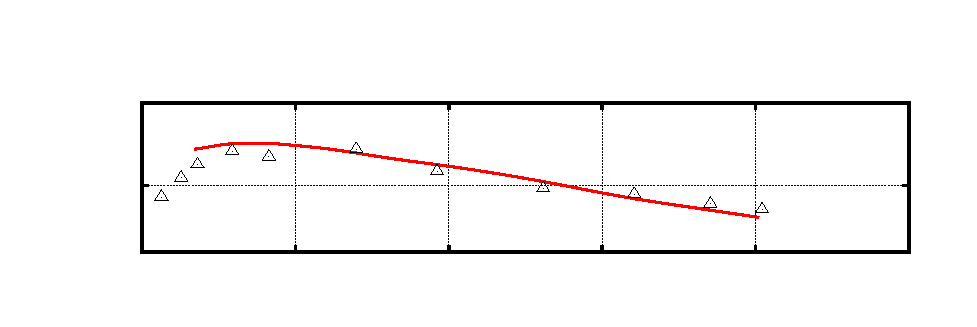
\includegraphics[width={453.50bp},height={141.70bp}]{nikitin1}}%
    \gplfronttext
  \end{picture}%
\endgroup
\\
 		% GNUPLOT: LaTeX picture with Postscript
\begingroup
  \makeatletter
  \providecommand\color[2][]{%
    \GenericError{(gnuplot) \space\space\space\@spaces}{%
      Package color not loaded in conjunction with
      terminal option `colourtext'%
    }{See the gnuplot documentation for explanation.%
    }{Either use 'blacktext' in gnuplot or load the package
      color.sty in LaTeX.}%
    \renewcommand\color[2][]{}%
  }%
  \providecommand\includegraphics[2][]{%
    \GenericError{(gnuplot) \space\space\space\@spaces}{%
      Package graphicx or graphics not loaded%
    }{See the gnuplot documentation for explanation.%
    }{The gnuplot epslatex terminal needs graphicx.sty or graphics.sty.}%
    \renewcommand\includegraphics[2][]{}%
  }%
  \providecommand\rotatebox[2]{#2}%
  \@ifundefined{ifGPcolor}{%
    \newif\ifGPcolor
    \GPcolorfalse
  }{}%
  \@ifundefined{ifGPblacktext}{%
    \newif\ifGPblacktext
    \GPblacktexttrue
  }{}%
  % define a \g@addto@macro without @ in the name:
  \let\gplgaddtomacro\g@addto@macro
  % define empty templates for all commands taking text:
  \gdef\gplbacktext{}%
  \gdef\gplfronttext{}%
  \makeatother
  \ifGPblacktext
    % no textcolor at all
    \def\colorrgb#1{}%
    \def\colorgray#1{}%
  \else
    % gray or color?
    \ifGPcolor
      \def\colorrgb#1{\color[rgb]{#1}}%
      \def\colorgray#1{\color[gray]{#1}}%
      \expandafter\def\csname LTw\endcsname{\color{white}}%
      \expandafter\def\csname LTb\endcsname{\color{black}}%
      \expandafter\def\csname LTa\endcsname{\color{black}}%
      \expandafter\def\csname LT0\endcsname{\color[rgb]{1,0,0}}%
      \expandafter\def\csname LT1\endcsname{\color[rgb]{0,1,0}}%
      \expandafter\def\csname LT2\endcsname{\color[rgb]{0,0,1}}%
      \expandafter\def\csname LT3\endcsname{\color[rgb]{1,0,1}}%
      \expandafter\def\csname LT4\endcsname{\color[rgb]{0,1,1}}%
      \expandafter\def\csname LT5\endcsname{\color[rgb]{1,1,0}}%
      \expandafter\def\csname LT6\endcsname{\color[rgb]{0,0,0}}%
      \expandafter\def\csname LT7\endcsname{\color[rgb]{1,0.3,0}}%
      \expandafter\def\csname LT8\endcsname{\color[rgb]{0.5,0.5,0.5}}%
    \else
      % gray
      \def\colorrgb#1{\color{black}}%
      \def\colorgray#1{\color[gray]{#1}}%
      \expandafter\def\csname LTw\endcsname{\color{white}}%
      \expandafter\def\csname LTb\endcsname{\color{black}}%
      \expandafter\def\csname LTa\endcsname{\color{black}}%
      \expandafter\def\csname LT0\endcsname{\color{black}}%
      \expandafter\def\csname LT1\endcsname{\color{black}}%
      \expandafter\def\csname LT2\endcsname{\color{black}}%
      \expandafter\def\csname LT3\endcsname{\color{black}}%
      \expandafter\def\csname LT4\endcsname{\color{black}}%
      \expandafter\def\csname LT5\endcsname{\color{black}}%
      \expandafter\def\csname LT6\endcsname{\color{black}}%
      \expandafter\def\csname LT7\endcsname{\color{black}}%
      \expandafter\def\csname LT8\endcsname{\color{black}}%
    \fi
  \fi
    \setlength{\unitlength}{0.0500bp}%
    \ifx\gptboxheight\undefined%
      \newlength{\gptboxheight}%
      \newlength{\gptboxwidth}%
      \newsavebox{\gptboxtext}%
    \fi%
    \setlength{\fboxrule}{0.5pt}%
    \setlength{\fboxsep}{1pt}%
    \definecolor{tbcol}{rgb}{1,1,1}%
\begin{picture}(9070.00,2834.00)%
    \gplgaddtomacro\gplbacktext{%
      \csname LTb\endcsname%%
      \put(1036,560){\makebox(0,0)[r]{\strut{}$0,6$}}%
      \csname LTb\endcsname%%
      \put(1036,1197){\makebox(0,0)[r]{\strut{}$1$}}%
      \csname LTb\endcsname%%
      \put(1036,1993){\makebox(0,0)[r]{\strut{}$1,5$}}%
      \csname LTb\endcsname%%
      \put(1204,280){\makebox(0,0){\strut{}$0$}}%
      \csname LTb\endcsname%%
      \put(2676,280){\makebox(0,0){\strut{}$0,2$}}%
      \csname LTb\endcsname%%
      \put(4148,280){\makebox(0,0){\strut{}$0,4$}}%
      \csname LTb\endcsname%%
      \put(5621,280){\makebox(0,0){\strut{}$0,6$}}%
      \csname LTb\endcsname%%
      \put(7093,280){\makebox(0,0){\strut{}$0,8$}}%
      \csname LTb\endcsname%%
      \put(8565,280){\makebox(0,0){\strut{}$1$}}%
    }%
    \gplgaddtomacro\gplfronttext{%
      \csname LTb\endcsname%%
      \put(266,1276){\rotatebox{-270}{\makebox(0,0){\strut{}$\bar{w}$}}}%
      \csname LTb\endcsname%%
      \put(4884,2413){\makebox(0,0){\strut{}$ i = 3\si\degree $}}%
    }%
    \gplbacktext
    \put(0,0){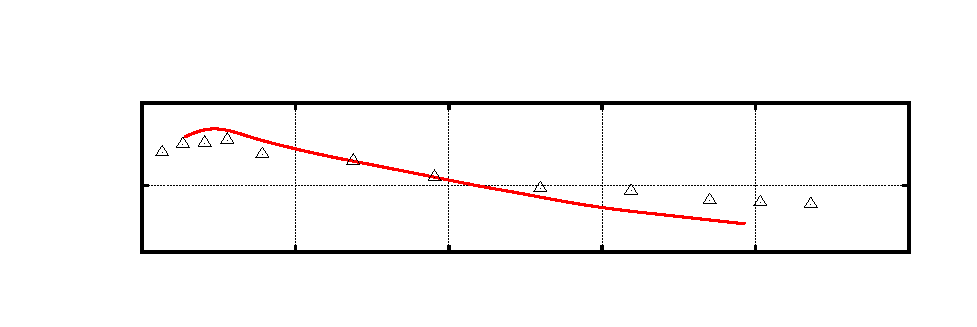
\includegraphics[width={453.50bp},height={141.70bp}]{nikitin2}}%
    \gplfronttext
  \end{picture}%
\endgroup
\\
 		% GNUPLOT: LaTeX picture with Postscript
\begingroup
  \makeatletter
  \providecommand\color[2][]{%
    \GenericError{(gnuplot) \space\space\space\@spaces}{%
      Package color not loaded in conjunction with
      terminal option `colourtext'%
    }{See the gnuplot documentation for explanation.%
    }{Either use 'blacktext' in gnuplot or load the package
      color.sty in LaTeX.}%
    \renewcommand\color[2][]{}%
  }%
  \providecommand\includegraphics[2][]{%
    \GenericError{(gnuplot) \space\space\space\@spaces}{%
      Package graphicx or graphics not loaded%
    }{See the gnuplot documentation for explanation.%
    }{The gnuplot epslatex terminal needs graphicx.sty or graphics.sty.}%
    \renewcommand\includegraphics[2][]{}%
  }%
  \providecommand\rotatebox[2]{#2}%
  \@ifundefined{ifGPcolor}{%
    \newif\ifGPcolor
    \GPcolorfalse
  }{}%
  \@ifundefined{ifGPblacktext}{%
    \newif\ifGPblacktext
    \GPblacktexttrue
  }{}%
  % define a \g@addto@macro without @ in the name:
  \let\gplgaddtomacro\g@addto@macro
  % define empty templates for all commands taking text:
  \gdef\gplbacktext{}%
  \gdef\gplfronttext{}%
  \makeatother
  \ifGPblacktext
    % no textcolor at all
    \def\colorrgb#1{}%
    \def\colorgray#1{}%
  \else
    % gray or color?
    \ifGPcolor
      \def\colorrgb#1{\color[rgb]{#1}}%
      \def\colorgray#1{\color[gray]{#1}}%
      \expandafter\def\csname LTw\endcsname{\color{white}}%
      \expandafter\def\csname LTb\endcsname{\color{black}}%
      \expandafter\def\csname LTa\endcsname{\color{black}}%
      \expandafter\def\csname LT0\endcsname{\color[rgb]{1,0,0}}%
      \expandafter\def\csname LT1\endcsname{\color[rgb]{0,1,0}}%
      \expandafter\def\csname LT2\endcsname{\color[rgb]{0,0,1}}%
      \expandafter\def\csname LT3\endcsname{\color[rgb]{1,0,1}}%
      \expandafter\def\csname LT4\endcsname{\color[rgb]{0,1,1}}%
      \expandafter\def\csname LT5\endcsname{\color[rgb]{1,1,0}}%
      \expandafter\def\csname LT6\endcsname{\color[rgb]{0,0,0}}%
      \expandafter\def\csname LT7\endcsname{\color[rgb]{1,0.3,0}}%
      \expandafter\def\csname LT8\endcsname{\color[rgb]{0.5,0.5,0.5}}%
    \else
      % gray
      \def\colorrgb#1{\color{black}}%
      \def\colorgray#1{\color[gray]{#1}}%
      \expandafter\def\csname LTw\endcsname{\color{white}}%
      \expandafter\def\csname LTb\endcsname{\color{black}}%
      \expandafter\def\csname LTa\endcsname{\color{black}}%
      \expandafter\def\csname LT0\endcsname{\color{black}}%
      \expandafter\def\csname LT1\endcsname{\color{black}}%
      \expandafter\def\csname LT2\endcsname{\color{black}}%
      \expandafter\def\csname LT3\endcsname{\color{black}}%
      \expandafter\def\csname LT4\endcsname{\color{black}}%
      \expandafter\def\csname LT5\endcsname{\color{black}}%
      \expandafter\def\csname LT6\endcsname{\color{black}}%
      \expandafter\def\csname LT7\endcsname{\color{black}}%
      \expandafter\def\csname LT8\endcsname{\color{black}}%
    \fi
  \fi
    \setlength{\unitlength}{0.0500bp}%
    \ifx\gptboxheight\undefined%
      \newlength{\gptboxheight}%
      \newlength{\gptboxwidth}%
      \newsavebox{\gptboxtext}%
    \fi%
    \setlength{\fboxrule}{0.5pt}%
    \setlength{\fboxsep}{1pt}%
    \definecolor{tbcol}{rgb}{1,1,1}%
\begin{picture}(9070.00,3968.00)%
    \gplgaddtomacro\gplbacktext{%
      \csname LTb\endcsname%%
      \put(1036,1456){\makebox(0,0)[r]{\strut{}$0,6$}}%
      \csname LTb\endcsname%%
      \put(1036,2199){\makebox(0,0)[r]{\strut{}$1$}}%
      \csname LTb\endcsname%%
      \put(1036,3127){\makebox(0,0)[r]{\strut{}$1,5$}}%
      \csname LTb\endcsname%%
      \put(1204,1176){\makebox(0,0){\strut{}$0$}}%
      \csname LTb\endcsname%%
      \put(2676,1176){\makebox(0,0){\strut{}$0,2$}}%
      \csname LTb\endcsname%%
      \put(4148,1176){\makebox(0,0){\strut{}$0,4$}}%
      \csname LTb\endcsname%%
      \put(5621,1176){\makebox(0,0){\strut{}$0,6$}}%
      \csname LTb\endcsname%%
      \put(7093,1176){\makebox(0,0){\strut{}$0,8$}}%
      \csname LTb\endcsname%%
      \put(8565,1176){\makebox(0,0){\strut{}$1$}}%
    }%
    \gplgaddtomacro\gplfronttext{%
      \csname LTb\endcsname%%
      \put(266,2291){\rotatebox{-270}{\makebox(0,0){\strut{}$\bar{w}$}}}%
      \put(4884,756){\makebox(0,0){\strut{}$\bar{x}$}}%
      \csname LTb\endcsname%%
      \put(7625,483){\makebox(0,0)[r]{\strut{}плоская решётка}}%
      \csname LTb\endcsname%%
      \put(7625,203){\makebox(0,0)[r]{\strut{}диагональная решётка}}%
      \csname LTb\endcsname%%
      \put(4884,3547){\makebox(0,0){\strut{}$ i = 7,8\si\degree $}}%
    }%
    \gplbacktext
    \put(0,0){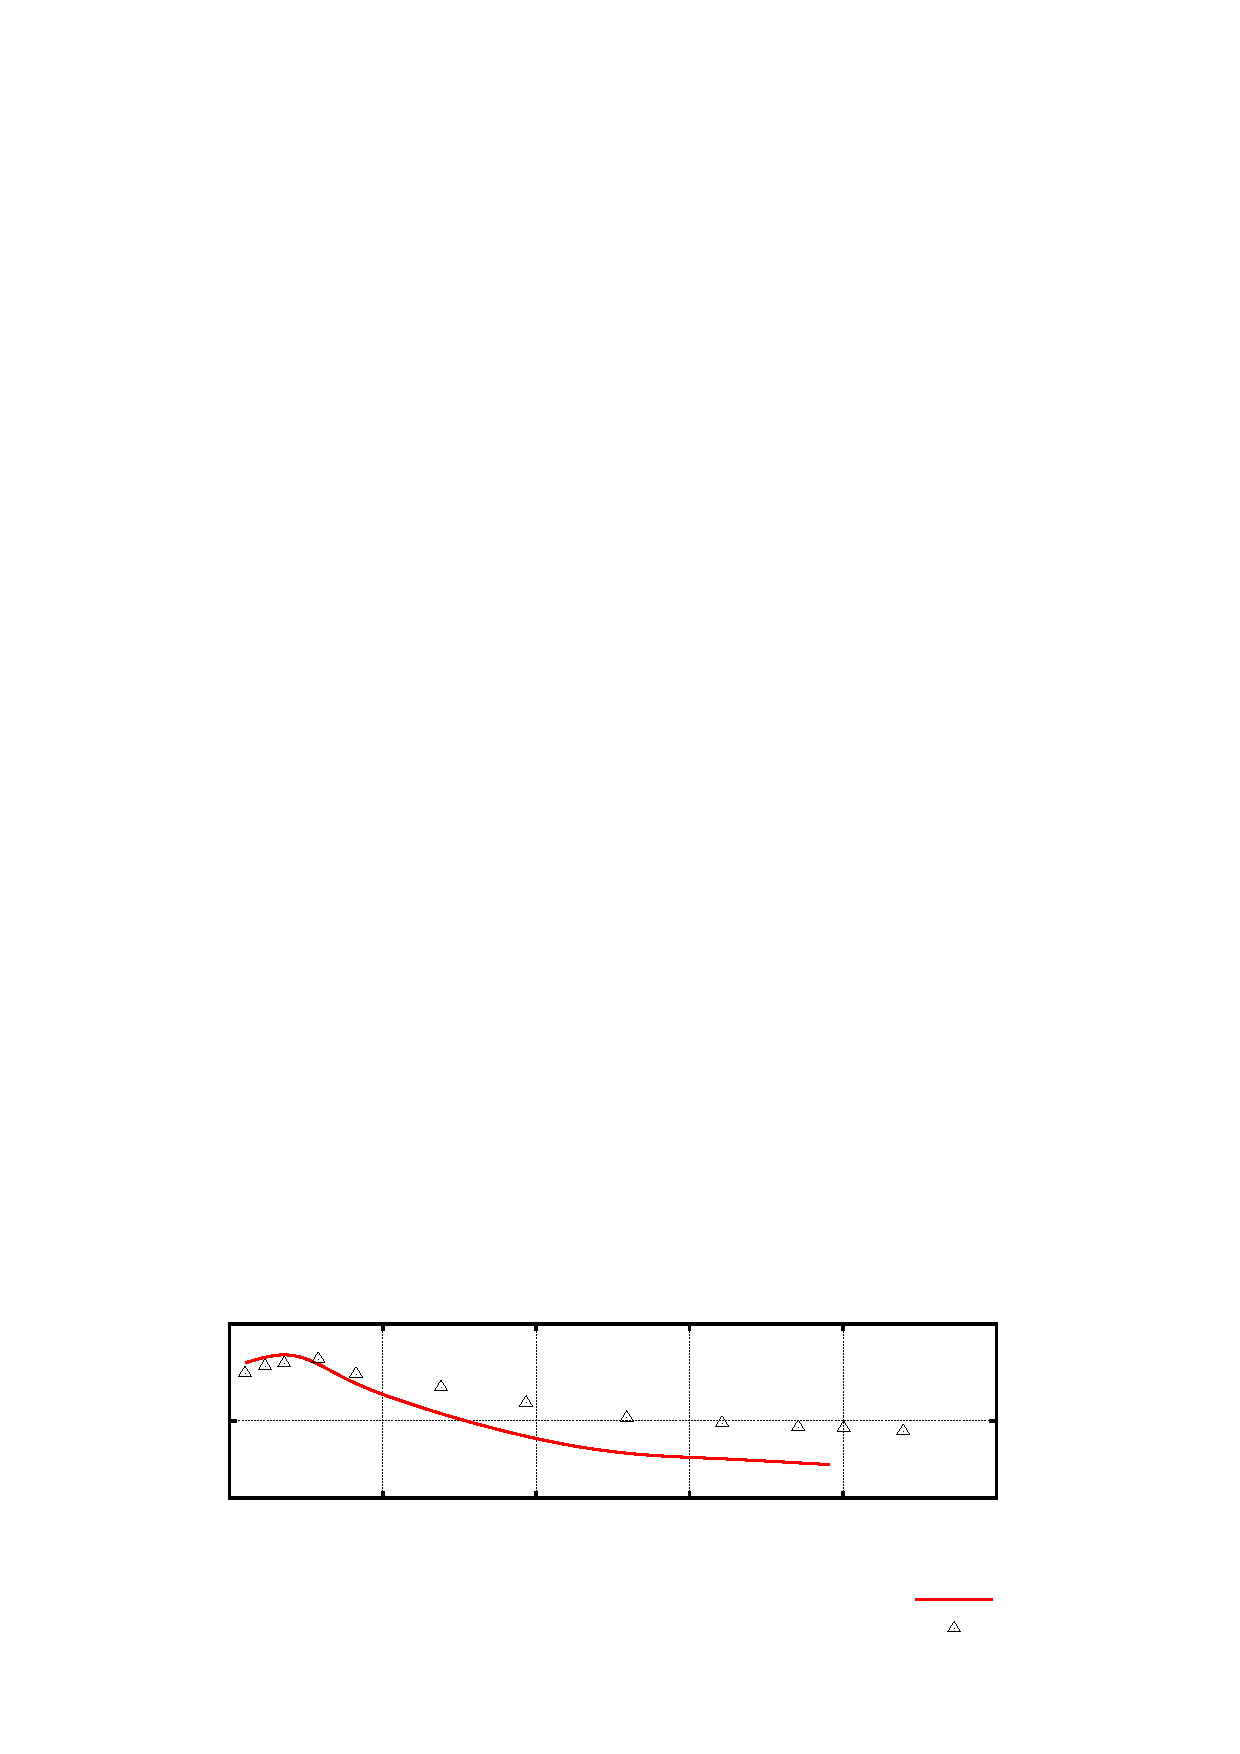
\includegraphics[width={453.50bp},height={198.40bp}]{nikitin3}}%
    \gplfronttext
  \end{picture}%
\endgroup

 	}
 	\caption{Сравнение распределений скоростей на спинке лопатки диагональной решётки и плоской \cite{Nikitin1966}} 
 	\label{fig:nikitin}
 \end{figure}
 
При рассмотрении течения во вращающейся пространственной решётке в относительной системе координат, в которой решётка остаётся неподвижной, поток является вихревым \cite{Jukovskiy1967,Viktorov1969}. Допущение о потенциальности течения в ядре потока перестаёт иметь смысл как и использование конформных отображений. Пересчёт данных продувок плоских профилей в таком случае становится неправомочным. Возможно использование теоретических характеристик, полученных, например, методами особенностей. Поток, при этом подходе, является наложением двух характерных потоков: бесциркуляционном обтекании неподвижной решётки профилей и движущейся решётки в отсутствии расхода.
 
Современные методы математического моделирования позволяют получить численное решение о вязком трёхмерном течении в проточной части рабочего колеса без использования сложных ограниченных моделей описанных выше, основываясь на более общих представлениях о законах течения. На данный момент, одним из основных подходов к созданию высокоэффективной компрессорной техники является численное трехмерное моделирование течения в проточной части, базирующееся на уравнениях Навье-Стокса, осреднённых по Рейнольдсу (CFD 3D RANS). Бурное развитие вычислительной техники в последние десятилетия и развитие универсальных программных комплексов, реализующих методы CFD 3D RANS, определило доминирующее положение этих методов в инженерных применениях. Через серии прямых задач решают задачи о проектировании турбомашин с меридиональным ускорением, обучая для этого нейронную сеть \cite{Bamberger2017}, или варьируя отдельные параметры для проектирования на конкретное задание \cite{Qiushi2010,Kim2018}. К сожалению, даже самые современные методы расчёта на высокопроизводительных вычислительных машинах не гарантируют получение решения, с достаточной точностью описывающего течение. К тому же нет общего метода моделирования течения в турбомашине. В зависимости от задачи, требуется применение различных граничных условий, моделей турбулентности и т.п. Данные полученные методами CFD 3D RANS, как и любыми другими расчётными методами, необходимо подтверждать в физическом эксперименте \cite{Michaud2016,Pandya2020}. 

\FloatBarrier
